\documentclass{article}

\author{Michael Cardiff}
\date{\today}

%% science symbols
\usepackage{amsmath,amssymb,amsthm}  % ams
\usepackage{siunitx}
\usepackage{bm,cancel}               % look nice
\usepackage{physics,slashed}         % phys specific

%% general pretty stuff
\usepackage{caption,float,graphicx,url,enumitem}
\usepackage{tikz,tikz-feynhand}
\usepackage{geometry}
\usepackage{booktabs}

% setup options
\captionsetup{labelfont=bf}
\geometry{margin=1in}

% macros
\renewcommand{\L}{\mathcal{L}}
\renewcommand{\H}{\mathcal{H}}
\renewcommand{\bar}{\overline}
\renewcommand{\l}{\ell}
\newcommand{\id}{\bm{1}}
\newcommand{\mcV}{\mathcal{V}}
\newcommand{\D}{\partial}
\newcommand{\M}{\mathcal{M}}
\newcommand{\veps}{\varepsilon}
\newcommand{\circled}[1]{\tikz[baseline=(char.base)]{
    \node[shape=circle,draw,inner sep=2pt](char){#1};}}

% mdframed environments
\usepackage[framemethod=TikZ]{mdframed}
\mdfsetup{skipabove=\topskip,skipbelow=\topskip}
\mdfdefinestyle{defstyle}{%
  linewidth=1pt,
  frametitlerule=true,
  frametitlebackgroundcolor=gray!40,
  backgroundcolor=gray!20,
  innertopmargin=\topskip
}

\mdfdefinestyle{todostyle}{%
  linewidth=0pt,
  frametitlerule=false,
  frametitlebackgroundcolor=red!40,
  backgroundcolor=red!20,
  innertopmargin=\topskip
}

\mdtheorem[style=defstyle]{definition}{Definition}
\mdtheorem[style=defstyle]{theorem}{Theorem}
\mdtheorem[style=defstyle]{problem}{Problem}
\mdtheorem[style=defstyle]{example}{Example}

\numberwithin{example}{section}

\newenvironment{thebook}
{\begin{mdframed}[style=defstyle,frametitle={From the Book}]}{\end{mdframed}}

\newenvironment{remark}
{\begin{mdframed}[style=defstyle,frametitle={Remark}]}{\end{mdframed}}

\newenvironment{TODO}
{\begin{mdframed}[style=todostyle,frametitle={TO DO}]}{\end{mdframed}}

\theoremstyle{plain}
\newtheorem*{note}{Note}
\newtheorem*{aside}{Aside}

\title{\vspace{-3em}Particle Physics Notes}
\date{\today}

% setups
\graphicspath{ {./figs/} }

\begin{document}
\maketitle

% -*- TeX-master: "master.tex" -*-
\section{Introduction}

Two important questions in physics:
\begin{itemize}
\item What is matter made of?
  \begin{itemize}
  \item What are the elementary constituents?
  \end{itemize}
\item How do the elementary constituents interact?
  \begin{itemize}
  \item What are the forces and dynamics in Nature?
  \end{itemize}
\end{itemize}

Most popular media focus on the first question. In Fermilab's ``search for the top quark'', or the LHC ``quest for the Higgs boson'', focus is placed on the excitement of discovering new forms of matter.

This is fun, but what is really exciting is not garnering a new trophy, but in what the existance of these new particles implies for the second question --- what new dynamics must exist that this new particle can help reveal?

\subsection{The matter}
\begin{itemize}
\item Hydrogen:
  \begin{figure}[H]
    \centering
    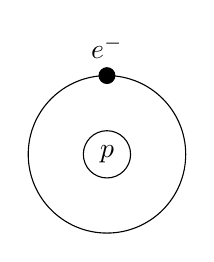
\begin{tikzpicture}{scale=1.5}
      \draw (0,0) circle [radius=0.3] node {$p$};
      \draw (0,0) circle [radius=1.0];
      \filldraw (0,1.0) circle [radius=0.1]
      node [yshift=1em] {$e^-$};
    \end{tikzpicture}
    \caption{Hydrogen Atom}
    \label{fig:hydrogen}
  \end{figure}
  A visualization is in fig~\ref{fig:hydrogen} Some properties of hydrogen:
  \begin{gather*}
    \text{Radius: } r_e\approx \SI{1}{\angstrom}\\
    \text{Binding Energy: }\SI{13}{\eV}
  \end{gather*}
  The unit of the binding energy is an Electron-Volt, which is what we will use for all energies for the duration of these notes.
  \begin{definition}[Electron-Volt]
    The electron volt is defined as the kinetic energy of an electron accelerated across a 1V potential, the usual SI unit prefixes can be applied such that 1keV=$10^3$eV, 1MeV=$10^6$eV etc.
  \end{definition}
\item Electron
  \begin{gather*}
    \text{Mass: } m_e= 0.511\text{ MeV}\\
    \text{Charge}=-1\\
    \text{Spin}=\frac12
  \end{gather*}
\item Proton
  \begin{gather*}
    \text{Mass: } m_p= 938\text{ MeV}\approx 1\text{ GeV}\\
    \text{Charge}=+1\\
    \text{Spin}=\frac12
  \end{gather*}
  \item Neutron
  \begin{gather*}
    \text{Mass: } m_n= m_p+1.3\text{ MeV}\approx m_p\\
    \text{Charge}=0\\
    \text{Spin}=\frac12
  \end{gather*}
  \item Deuterium is a Hydrogen with a neutron
\end{itemize}

\paragraph{Sizes}
\begin{itemize}
\item The electron is effectively a point
\item The nucleons, which are protons and neutrons have a ``radius'' of $\sim 10^{-15}$m, which is given the name of $1$fm, a ``Fermi'' or femtometer, which is notably less than the scale of hydrogen
\end{itemize}

\subsection{Forces in play:}
\begin{itemize}
\item Gravity $\sim$ negligible:
  \begin{align*}
    F=G_N\frac{m_p m_e}{r^2}
  \end{align*}
\item Electric:
  \begin{align*}
    F=\frac{e^2}{4\pi}\frac{Q_p Q_e}{r^2}
  \end{align*}
\item Strong --- Binds nucleons into nuclei
\item Weak --- Causes nuclear ``beta'' decay, and fusion
\end{itemize}

\subsection{Beta ($\beta$) decay}
A Process described by:
\begin{align*}
  n\to p+e^{-}+\bar{\nu}_e
\end{align*}
Where $\bar{\nu}_e$ is an anti-electron neutrino. This process has a lifetime $\tau$ of $14$ minutes.

Note that $m_n-m_p>m_e$

\paragraph{Q/ Why doesn't deuterium decay?} In short, conservation of energy, since $2m_p+m_e+m_{\nu_e}=1877.05$MeV, however, the mass of deuterium is $m_d=1876.64$. The masses are not large enough to allow for this decay:
\begin{figure}[H]
  \centering
  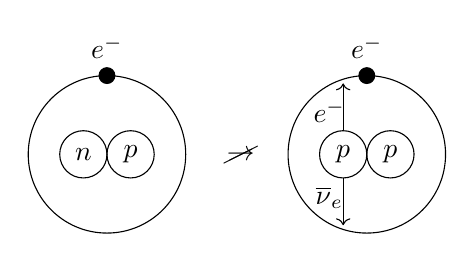
\begin{tikzpicture}
    \draw (0,0) circle [radius=0.3] node {$n$};
    \draw (0.6,0) circle [radius=0.3] node {$p$};
    \draw (0.3,0) circle [radius=1.0];
    \filldraw (0.3,1.0) circle [radius=0.1]
    node [yshift=1em] {$e^-$};
    \node at (2.0,0) {$\cancel{\rightarrow}$};
    \draw (3.3,0) circle [radius=0.3] node {$p$};
    \draw (3.9,0) circle [radius=0.3] node {$p$};
    \draw (3.6,0) circle [radius=1.0];
    \filldraw (3.6,1.0) circle [radius=0.1]
    node [yshift=1em] {$e^-$};
    \draw[->] (3.3,-0.3) to (3.3,-0.9) node [yshift=1em] {\hspace{-1em}$\bar{\nu}_e$};
    \draw[->] (3.3,0.3) to (3.3,0.9) node [yshift=-1em] {\hspace{-1em}$e^{-}$};
  \end{tikzpicture}
  \caption{Theoretical Deuterium Decay}
\end{figure}

\paragraph{Neutrinos and $\beta$ decay}
The other interesting story of $\beta$ decay is regarding the neutrino. In 1930, Chadwick observed the decay of tritium: $^3$H $\to\ ^3$He$+e^-$. Strangely, the $e^-$ was \emph{not} monoenergetic, as conservation of energy and momentum would require. This was catastrophic, and confronted with experimental evidence, many were prepared to throw out energy conservation. Pauli proposed a ``desperate remedy'' that some invisible particle must be carrying the energy away. Fermi's theory of weak interactions described this particle as a ``neutrino'' (little neutral one), and successfully described $\beta$ decay.

\textbf{Note}: The neutrino in $\beta$ decay was later found to be an antiparticle.

\begin{itemize}
\item Neutrinos then can be added to our list of ``matter''
  \begin{align*}
    \SI{0.01}{\eV}\leq m_{\nu_e}\leq\SI{1.4}{\eV}
  \end{align*}
  A consequence of this mass is that we can take neutrinos to be kinematically massless.
\end{itemize}

\subsection{Antiparticles}
Every particle has an antiparticle with opposite quantum numbers, but identical mass and spin:
\begin{itemize}
\item The electron $e^-$ has the positron $e^+$
\item The proton $p$ has the antiproton $\bar{p}$
\item The neutron $n$ has the antineutron $\bar{n}$
\item And the neutrinos $\nu$ have the antineutrinos $\bar{\nu}$ as we have seen
\end{itemize}
These (specifying the electron neutrino and its antiparticle) compose $\sim100\%$ of all the \textbf{observed} matter in the universe, though are only $5\%$ of the total matter.

Up to this point we have used chemistry and nuclear physics, particle physics picks up at the next level of depth.

\subsection{Quarks}
As it turns out, the proton and neutron are \textbf{not} fundamental.

If you perform a Rutherford-like scattering experiment at large energies (short distance), you find that protons and neutrons are composed of 3 hard spheres, called ``constituent quarks''

In fact, we go a bit deeper and find:
\begin{itemize}
\item The up quark $u$ and the up antiquark $\bar{u}$
\item The down quark $d$ and the down antiquark $\bar{d}$
\end{itemize}

These were ``predicted'' by Gell-Mann and Zweig as an explanation for apparent relationships between other particles, but we are getting ahead of ourselves.

The new particles we can add to our list of matter is:

\begin{itemize}
\item Up quark
  \begin{gather*}
    \text{Mass: } m_u= 4\text{ MeV} \ll m_p\\
    \text{Charge}=+\frac23\\
    \text{Spin}=\frac12
  \end{gather*}
\item Down quark
  \begin{gather*}
    \text{Mass: } m_d= 7\text{ MeV} \ll m_p\\
    \text{Charge}=-\frac13\\
    \text{Spin}=\frac12
  \end{gather*}
\end{itemize}
Note the odd fractional charge that both of these quarks have.

We can then think of $p,\bar{p}$ and $n,\bar{n}$ as:
\begin{figure}[H]
  \centering
  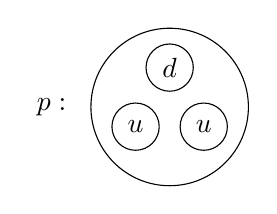
\begin{tikzpicture}
    \node at (0,0) {$p:$};
    \draw (1.500, 0.00) circle (1.0);
    \draw (1.500, 0.50) circle (0.3) node {$d$};
    \draw (1.067,-0.25) circle (0.3) node {$u$};
    \draw (1.933,-0.25) circle (0.3) node {$u$};
  \end{tikzpicture}
  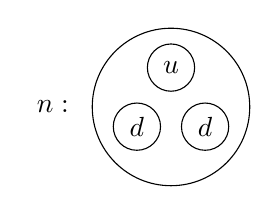
\begin{tikzpicture}
    \node at (0,0) {$n:$};
    \draw (1.500, 0.00) circle (1.0);
    \draw (1.500, 0.50) circle (0.3) node {$u$};
    \draw (1.067,-0.25) circle (0.3) node {$d$};
    \draw (1.933,-0.25) circle (0.3) node {$d$};
  \end{tikzpicture}
  \\
  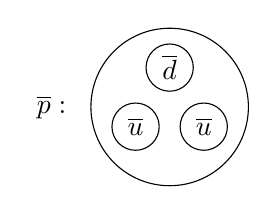
\begin{tikzpicture}
    \node at (0,0) {$\bar{p}:$};
    \draw (1.500, 0.00) circle (1.0);
    \draw (1.500, 0.50) circle (0.3) node {$\bar{d}$};
    \draw (1.067,-0.25) circle (0.3) node {$\bar{u}$};
    \draw (1.933,-0.25) circle (0.3) node {$\bar{u}$};
  \end{tikzpicture}
  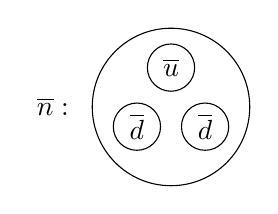
\begin{tikzpicture}
    \node at (0,0) {$\bar{n}:$};
    \draw (1.500, 0.00) circle (1.0);
    \draw (1.500, 0.50) circle (0.3) node {$\bar{u}$};
    \draw (1.067,-0.25) circle (0.3) node {$\bar{d}$};
    \draw (1.933,-0.25) circle (0.3) node {$\bar{d}$};
  \end{tikzpicture}
  \caption{Protons and Neutrons as Quarks}
\end{figure}

\subsection{Beta Decay Again}
We should revisit $\beta$ decay in terms of the constituent quarks of protons and neutrons. We instead see the process as:
\begin{figure}[H]
  \centering
  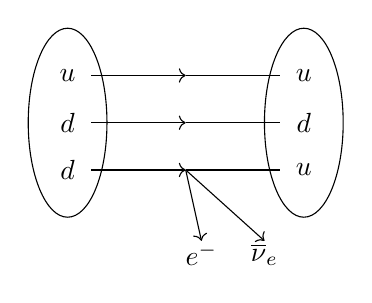
\begin{tikzpicture}
    \draw (0,0) ellipse (0.5 and 1.2);
    \node at (0, 0.6) {$u$};
    \node at (0, 0.0) {$d$};
    \node at (0,-0.6) {$d$};
    \draw (3,0) ellipse (0.5 and 1.2);
    \node at (3, 0.6) {$u$};
    \node at (3, 0.0) {$d$};
    \node at (3,-0.6) {$u$};
    \draw[->] (0.3, 0.6) to (1.5, 0.6);
    \draw[-]  (1.5, 0.6) to (2.7, 0.6);
    \draw[->] (0.3, 0.0) to (1.5, 0.0);
    \draw[-]  (1.5, 0.0) to (2.7, 0.0);
    \draw[->] (0.3,-0.6) to (1.5,-0.6);
    \draw[-]  (1.5,-0.6) to (2.7,-0.6);
    \draw[->] (1.5,-0.6) to (1.7,-1.5) node [yshift=-0.5em] {$e^-$};
    \draw[->] (1.5,-0.6) to (2.5,-1.5) node [yshift=-0.5em] {$\bar{\nu}_e$};
  \end{tikzpicture}
  \caption{$\beta$ decay in terms of quarks}
  \label{fig:beta}
\end{figure}
Thus we can describe the Fermi weak interaction in terms of quarks:
\begin{figure}[H]
  \centering
  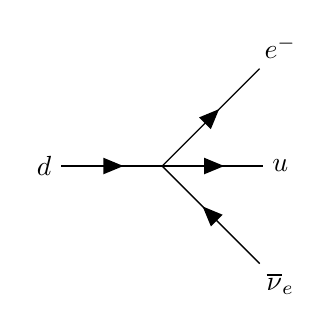
\begin{tikzpicture}
    \begin{feynhand}
      \vertex (a) at (0,0) {$d$};
      \vertex (i) at (1.5,0);
      \vertex (b) at (3,0) {$u$};
      \vertex (e) at (3,1.5) {$e^-$};
      \vertex (n) at (3,-1.5) {$\bar{\nu}_e$};
      \propag[fer] (a) to (i);
      \propag[fer] (i) to (b);
      \propag[fer] (i) to (e);
      \propag[antfer] (i) to (n);
    \end{feynhand}
  \end{tikzpicture}
  \caption{``Four-Fermion'' Fermi Interaction}
  \label{fig:fermi}
\end{figure}

Thus so far, our ``Standard Model'' looks just like:
\begin{gather*}
  \pmqty{u\\d}\\
  \pmqty{\nu_e\\e}
\end{gather*}

However, there is still more to come!

\subsection{Muon}
Denoted by $\mu^\pm$. In 1937 Neddermeyer and Anderson, and Street and Stevenson, found muons in showers of cosmic rays (particles hit the upper atmosphere, and produce heavy charged particles that reach the ground). Originally, they were thought to be particles predicted by Yukawa to mediate the strong force because their mass, $\SI{105}{\mega\eV}$ is close to that of the now known pion, $m_\pi\approx\SI{139}{\mega\eV}$. They were (poorly) called ``mu meons''.

The dominant decay of a muon suggests a 3-bpdyy decay:
\begin{align*}
  \mu^+\to e^+\nu_e\bar{\nu}_{?}
\end{align*}
The lack of observation of $\mu^+\to e^+\gamma$, and later in 1962 at the AGS, where Lederman, Schwartz, and Steinberger showed $\bar{\nu}_\mu+p\to\mu^++n$, but $\bar{\nu}+p\cancel{\to}e^++n$, in the inverse reaction, implied the existance of a muon neutrino.

\subsection{The Zoo}
By 1961, there were 27 ``fundamental'' strongly interacting particles known. Gell-Mann and Ne'eman independently noticed that adding a ``strange'' new quantum number, they could collect the particles into groups related by a simple symmetry --- $SU(3)$, which we'll discuss later.

By 1964, only one particle was missing --- one with 3 units of ``strangeness'':
\begin{figure}[H]
  \centering
  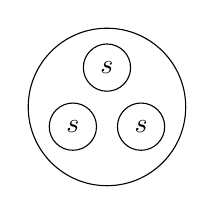
\begin{tikzpicture}
    \draw (1.500, 0.00) circle (1.0);
    \draw (1.500, 0.50) circle (0.3) node {$s$};
    \draw (1.067,-0.25) circle (0.3) node {$s$};
    \draw (1.933,-0.25) circle (0.3) node {$s$};
  \end{tikzpicture}
  \caption{Theoretical ``Strange'' Particle}
  \label{fig:strange}
\end{figure}
This particle is predicted to have spin $\frac32$ and charge $-1$. They also preduced the mass $\SI{1.7}{\giga\eV}$, and lifetime. In 1964, the $\Omega^-$ was discovered at Brookhaven National Lab.

\begin{itemize}
\item The effects of this new periodic table called ``The Eightfold Way'' were profound. The concept of symmetry as \emph{the} central theoretical device was established --- and we are still paying that price\ldots
\item Later Gell-Mann and Zweig proposed the quark model of 3 flavors: up, down, strange. By 1970 this model was in trouble.
\item Free quarks had not been observed.
\item The weak decay $s\cancel{\to}d\nu\bar{\nu}$ did not appear. Glashow, Iliopoulos, and Maiani proposed a ``charming'' solution to the latter. Adding a fourth quark with charge $+\frac23$ would allow for a symmetry to forbid these ``neutral current'' decays. 
\item In 1974 BNL and SLAC each discovered a $c\bar{c}$-bound state, called the $J/\psi$. The lifetime of $\SI{e-20}{\s}$ was 1000 times longer than for strange particles.
\item It seemed clear that the number of quarks $=$ the number of leptons
\end{itemize}
This gives a new standard model:
\begin{gather*}
  \pmqty{u\\d}\quad\qquad\pmqty{c\\s}\\
  \underbrace{\pmqty{\nu_e\\e}}_{1^{\text{st}}\text{ Generation}}
  \underbrace{\pmqty{\nu_\mu\\\mu}}_{2^{\text{nd}}\text{ Generation}}
\end{gather*}
The new additions are:
\begin{itemize}
\item Charm quark: $m_c\approx\SI{1.25}{\GeV}\gg m_u$
\item Strange quark: $m_d\approx\SI{95}{\MeV}\gg m_d$
\item Muon: $m_\mu=\SI{105.658369}{\MeV}\gg m_e$
\item Muon neutrino: $m_{\nu_\mu}\approx m_{\nu_e}\approx0$
\end{itemize}

The second generation particles are \emph{unstable}:
\begin{figure}[H]
  \centering
  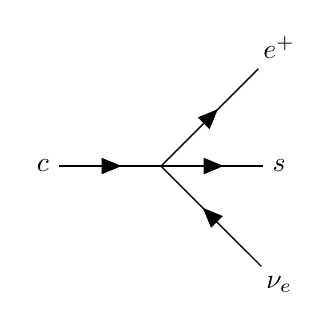
\begin{tikzpicture}
    \begin{feynhand}
      \vertex (a) at (0,0) {$c$};
      \vertex (i) at (1.5,0);
      \vertex (b) at (3,0) {$s$};
      \vertex (e) at (3,1.5) {$e^+$};
      \vertex (n) at (3,-1.5) {$\nu_e$};
      \propag[fer] (a) to (i);
      \propag[fer] (i) to (b);
      \propag[fer] (i) to (e);
      \propag[antfer] (i) to (n);
    \end{feynhand}
  \end{tikzpicture}
  \begin{tikzpicture}
    \begin{feynhand}
      \vertex (a) at (0,0) {$c$};
      \vertex (i) at (1.5,0);
      \vertex (b) at (3,0) {$s$};
      \vertex (e) at (3,1.5) {$\mu^+$};
      \vertex (n) at (3,-1.5) {$\nu_\mu$};
      \propag[fer] (a) to (i);
      \propag[fer] (i) to (b);
      \propag[fer] (i) to (e);
      \propag[antfer] (i) to (n);
    \end{feynhand}
  \end{tikzpicture}
  \\
  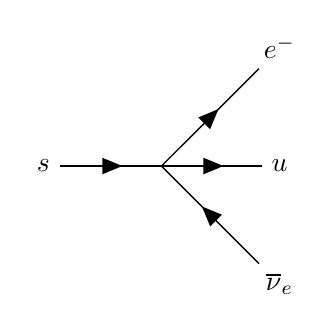
\begin{tikzpicture}
    \begin{feynhand}
      \vertex (a) at (0,0) {$s$};
      \vertex (i) at (1.5,0);
      \vertex (b) at (3,0) {$u$};
      \vertex (e) at (3,1.5) {$e^-$};
      \vertex (n) at (3,-1.5) {$\bar{\nu}_e$};
      \propag[fer] (a) to (i);
      \propag[fer] (i) to (b);
      \propag[fer] (i) to (e);
      \propag[antfer] (i) to (n);
    \end{feynhand}
  \end{tikzpicture}
  \begin{tikzpicture}
    \begin{feynhand}
      \vertex (a) at (0,0) {$s$};
      \vertex (i) at (1.5,0);
      \vertex (b) at (3,0) {$u$};
      \vertex (e) at (3,1.5) {$\mu^-$};
      \vertex (n) at (3,-1.5) {$\bar{\nu}_\mu$};
      \propag[fer] (a) to (i);
      \propag[fer] (i) to (b);
      \propag[fer] (i) to (e);
      \propag[antfer] (i) to (n);
    \end{feynhand}
  \end{tikzpicture}
  \\
  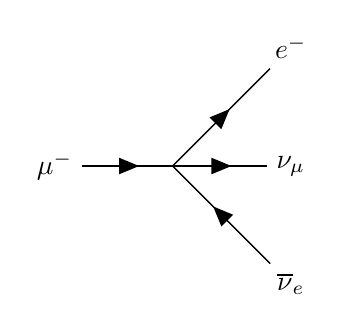
\begin{tikzpicture}
    \begin{feynhand}
      \vertex (a) at (0,0) {$\mu^-$};
      \vertex (i) at (1.5,0);
      \vertex (b) at (3,0) {$\nu_\mu$};
      \vertex (e) at (3,1.5) {$e^-$};
      \vertex (n) at (3,-1.5) {$\bar{\nu}_e$};
      \propag[fer] (a) to (i);
      \propag[fer] (i) to (b);
      \propag[fer] (i) to (e);
      \propag[antfer] (i) to (n);
    \end{feynhand}
  \end{tikzpicture}
  \caption{Second Generation Decays}
  \label{fig:gentwo}
\end{figure}
In 1975 the $\tau$ lepton was discovered at SLAC in $e^+e^-\to\tau^+\tau^-$. Immediate searches began for third generation particles:
\begin{itemize}
\item 2001 DONUT at Fermilab observed $\nu_\tau$ events in emulsion
\item 1977 a $b\bar{b}$-bound state called the upsilon was discovered at Fermilab, $m_b\approx\SI{5}{\GeV}$
\item There \emph{had} to be a sixth quark of mass $m_t<\SI{45}{\GeV}$, no $\SI{80}{\GeV}$, no $\SI{110}{\GeV}$, no $\SI{140}{\GeV}$. WHERE IS IT???
\item 1995 top quark discovered at Fermilab via its decay. Lifetime so short it forms \emph{no} bound states! $m_t\approx\SI{175}{\GeV}$. 
\end{itemize}
Thus we have the third generation:
\begin{gather*}
  \pmqty{u\\d}\hspace{0.5em}\pmqty{c\\s}\hspace{0.5em}\pmqty{t\\b}\\
  \pmqty{\nu_e\\e}\pmqty{\nu_\mu\\\mu}\pmqty{\nu_\tau\\\tau}
\end{gather*}
New additions:
\begin{itemize}
\item Top quark: $m_t=\SI{172.4}{\GeV}$
\item Bottom quark: $m_b=\SI{4.5}{\GeV}$
\item Tau: $m_\tau=\SI{1.78}{\GeV}$
\item Tau neutrino: $m_{\nu_\tau}\approx m_{\nu_e}\approx m_{\nu_\mu}\leq \SI{1}{\eV}$
\end{itemize}

\paragraph{Fourth Generation?}

There is no evidence for a fourth generation current, but if there were, we would expect:
\begin{gather*}
  m_{\nu_4}>40-\SI{45}{\GeV}\\
  m_{\ell_4}\geq\SI{100}{\GeV}\\
  m_{b'}\geq\SI{130}{\GeV}
\end{gather*}

\paragraph{Great Mysteries:}

\begin{itemize}
\item Why are there 3 generations?
\item Why do some mix and others not?
\item Why do masses range from $10^{-12}$ to $10^2$ \si{\GeV}?
\end{itemize}

\subsection{Forces (Interactions):}
Relativity and quantum mechanics lead to Quantum Field Theory.

There are 4 forces at play (kinda):
\begin{enumerate}
  \setcounter{enumi}{-1}
\item \emph{Gravity}, as mentioned, is simply too weak at the level of particles to observe. Therefore we'll ignore it (for now).
\item \emph{Electromagnetism}: Mediated by exchange of virtual bosons called photons, $\gamma$:
  \begin{gather*}
    \text{Mass: } m_\gamma= 0\\
    \text{Charge}=0\\
    \text{Spin}=1
  \end{gather*}
  Einstein's Nobel Prize was not for gravity, but for this 1905 argument that the electromagnetic field was quantized. Hence, light really could be though of as a particle with energy $E=h\nu$, and not just as a wave.

  In 1923, Compton showed that light scattered from a particle of mass $m$ had a wavelength shifted by $\lambda-\lambda'=\lambda_c(1-\cos\theta)$, with $\lambda_c=\frac{h}{mc}$-precisely what you get if $m_\gamma=0$ and is a particle.

  Photons (light) couple to anything that carries charge. So far that is $e^\pm$, $u$, $d$, $\bar{u}$, $\bar{d}$, and other generations.
\item \emph{Strong Force}: Mediated by gluons, $g$:
    \begin{gather*}
    \text{Mass: } m_g= 0\\
    \text{Charge}=0\\
    \text{Spin}=1
  \end{gather*}
  Quarks feel gluon force, leptons do not.

  Quarks carry \emph{color}=red, green, blue.

  Gluons have to bind strongly to overcome EM repulsion. They save the quark model by saying there are actually 3 quarks for each type: $u,d,s$ etc. Otherwise the $\Omega^-(sss)$  could not exist due to the Pauli exclusion principle. When $\Omega^-$ was found in 1964, Greenberg proposed the color model. There were strong lingering doubts about this solution until 1979 where PETRA at DESY produced 3 jets: $q,\bar{q},g$.

  \emph{Note}: There are 9 color combinations, but only 8 gluons, we'll return.
\item \emph{Weak Force}: Mediated by massive $W/Z$ Bosons.

  What we earlier called the ``Fermi interaction'' is really exchange of a heavy particle. Force is not intrinsically weak, just suppressed by $W$ mass:
  \begin{gather*}
    \text{Mass: } m_W= \SI{80.4}{\GeV}\\
    \text{Charge}=\pm1\\
    \text{Spin}=1
  \end{gather*}
  $W$ boson changed particle type or \emph{flavor}
\end{enumerate}

The underlying field theories behind each of these has a name:
\begin{itemize}
\item Electromagnetism: Quantum Electro Dynamics (QED)
\item Strong Force: Quantum Chromo Dynamics (QCD)
\item Weak Force: Quantum Flavor Dynamics (QFD)\footnote{This nomenclature however is rarely used.}
\end{itemize}
The Standard Model is described by \emph{Gauge Theory}, QED, QCD and QFD are all examples of gauge theories, based on ``local'' symmetries.

A gauge theory is described by a gauge ``group''
\begin{itemize}
\item QED
  \begin{align*}
    u\to \underbrace{e^{i\theta}}_{U(1)}u
  \end{align*}
  
\item QFD
  \begin{align*}
    \pmqty{u\\d}\to \underbrace{\pmqty{&&& \\ &&&}}_{2\times2:SU(2)}\pmqty{u\\d}
  \end{align*}
\item QCD
  \begin{align*}
    \pmqty{u_r\\u_g\\u_b}\to
    \underbrace{\pmqty{&&&&& \\ &&&&& \\ &&&&&}}_{3\times3:SU(3)}
    \pmqty{u_r\\u_g\\u_b}
  \end{align*}
\end{itemize}
Particles (fields) experience forces described by their transformation under these groups.

The Standard model group is: $SU(3)\times SU(2)\times U(1)$

Note that Gravity is \emph{not} a gauge theory.

There are two types of symmetry we would like to include in our theory of the universe, global and local ones.
\begin{definition}[Global Symmetry]
  A global symmetry is a symmetry that changes every point in the transformation space the same. For a rotation, the entire system would be shifted by some angle $\theta$.
\end{definition}
Global symmetries, while nice, give rise to a sort of action at a distance, which is something we want to avoid in our interpretation of the universe via Field Theory. This leads to a sense that the symmetries of the Standard Model are ``Local'' rather than global, hence the other type of symmetry to discuss
\begin{definition}[Local Symmetry]
  A non global symmetry is called a local symmetry, and is characterized by the transformation parameter having dependence on spacetime:
  \begin{gather*}
    \text{Global Parameter: }\theta\\
    \text{Local  Parameter: }\theta(x)
  \end{gather*}
\end{definition}

A Gauge theory is a theory of massless spin-one particles that transmit force.
\begin{itemize}
\item QED: $m_\gamma=0$
\item QCD: $m_g=0$
\item QFD: $M_W=\SI{80.4}{\GeV}$, whoops!
\end{itemize}
The Gauge Symmetry is apparently \emph{broken} (or Hidden).

\begin{remark}
  An analogous system is a ferromagnet:
  \begin{figure}[H]
    \centering
    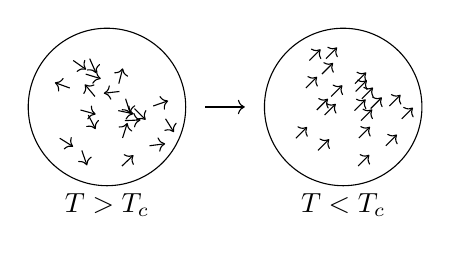
\begin{tikzpicture}
      \node at (0,-1.25) {$T>T_c$};
      \draw (0,0) circle (1.0);
      \draw[->] (0.34954, -0.0199438) to (0.490203, -0.162119);
      \draw[->] (0.150047, 0.296553) to (0.20043, 0.490102);
      \draw[->] (0.743747, -0.150205) to (0.850037, -0.319624);
      \draw[->] (0.198332, -0.393883) to (0.258539, -0.203161);
      \draw[->] (-0.335555, -0.038404) to (-0.14284, -0.0918898);
      \draw[->] (-0.152624, 0.13327) to (-0.281111, 0.286538);
      \draw[->] (0.236579, 0.104484) to (0.29672, -0.0862591);
      \draw[->] (-0.319563, -0.55186) to (-0.253705, -0.740706);
      \draw[->] (0.226788, -0.173314) to (0.426614, -0.164954);
      \draw[->] (-0.472952, 0.240987) to (-0.660934, 0.309271);
      \draw[->] (-0.428682, 0.59036) to (-0.265005, 0.475426);
      \draw[->] (0.143533, -0.0461538) to (0.339274, -0.0872084);
      \draw[->] (0.540831, -0.492648) to (0.739169, -0.466921);
      \draw[->] (-0.270044, 0.417371) to (-0.0786918, 0.359195);
      \draw[->] (-0.236663, -0.102218) to (-0.145731, -0.28035);
      \draw[->] (-0.599859, -0.396888) to (-0.430448, -0.50319);
      \draw[->] (0.190446, -0.749809) to (0.335538, -0.612156);
      \draw[->] (0.587397, 0.0124832) to (0.776281, 0.078231);
      \draw[->] (-0.219336, 0.613831) to (-0.138749, 0.430786);
      \draw[->] (0.158473, 0.196568) to (-0.0402765, 0.174242);
      \draw (3,0) circle (1.0);
      \node at (3,-1.25) {$T<T_c$};
      \draw[->] (3.34954, -0.0199438) to (3.49096, 0.121478);
      \draw[->] (3.15005, 0.296553) to (3.29147, 0.437974);
      \draw[->] (3.74375, -0.150205) to (3.88517, -0.00878408);
      \draw[->] (3.19833, -0.393883) to (3.33975, -0.252462);
      \draw[->] (2.66444, -0.038404) to (2.80587, 0.103017);
      \draw[->] (2.84738, 0.13327) to (2.9888, 0.274691);
      \draw[->] (3.23658, 0.104484) to (3.378, 0.245906);
      \draw[->] (2.68044, -0.55186) to (2.82186, -0.410439);
      \draw[->] (3.22679, -0.173314) to (3.36821, -0.0318922);
      \draw[->] (2.52705, 0.240987) to (2.66847, 0.382408);
      \draw[->] (2.57132, 0.59036) to (2.71274, 0.731782);
      \draw[->] (3.14353, -0.0461538) to (3.28495, 0.0952676);
      \draw[->] (3.54083, -0.492648) to (3.68225, -0.351226);
      \draw[->] (2.72996, 0.417371) to (2.87138, 0.558792);
      \draw[->] (2.76334, -0.102218) to (2.90476, 0.0392038);
      \draw[->] (2.40014, -0.396888) to (2.54156, -0.255467);
      \draw[->] (3.19045, -0.749809) to (3.33187, -0.608388);
      \draw[->] (3.5874, 0.0124832) to (3.72882, 0.153905);
      \draw[->] (2.78066, 0.613831) to (2.92209, 0.755253);
      \draw[->] (3.15847, 0.196568) to (3.29989, 0.33799);
      \draw[->] (1.25,0) to (1.75,0);
    \end{tikzpicture}
    \caption{Ferromagnet Symmetry Breaking}
    \label{fig:magnet}
  \end{figure}
  For $T>T_c$, there is clearly no preferred direction for the system, so for all intents and purposes it is rotationally symmetric. However as soon as we go below $T_c$, this symmetry is ``spontaneously'' broken.
\end{remark}

We do not know what ``breaks'' the symmetry $\implies$ \underline{new force of nature}.

The central question in particle physics today is to answer what new force exists, and what are the particles associated with it?

A second frontier: What is the origin of quark and lepton masses?

\subsection{Units in Particle Physics}
\begin{table}[H]
  \centering
  \begin{tabular}{c|c}
    Typical Energies & Sizes\\ \hline
    \si{\eV} $\sim10^{1} \si{\eV}$ & $\si{\nm}\sim10^{-9}\si{\m}$  \\
    \si{\keV}$\sim10^{3} \si{\eV}$ & $\si{\angstrom}\sim10^{-10}\si{\m}$  \\
    \si{\MeV}$\sim10^{6} \si{\eV}$ & $\si{\pm}\sim10^{-12}\si{\m}$  \\
    \si{\GeV}$\sim10^{9} \si{\eV}$ & $\si{\femto\m}\sim10^{-15}\si{\m}$  \\
    \si{\TeV}$\sim10^{12}\si{\eV}$
  \end{tabular}
  \caption{Typical Values in Particle Physics}
\end{table}

\begin{definition}[Natural Units]
  As a convention, factors of $\hbar$ and $c$ are set to be $1$, meaning they are dimensionless as well as valueless, so everything is measired in units of energy.

  The only conversion factors we need to know:
  \begin{align*}
    c&=\SI{3e8}{\m\per\s}\\
    \hbar c&=\SI{197}{\MeV\femto\m}
  \end{align*}
  These are the only values we need to memorize.
\end{definition}

Electric charge can get complicated with most authors either using Lorentz-Heaviside units:
\begin{align*}
  F=\frac{e^2}{4\pi}\frac{Q_e Q_p}{r^2}
\end{align*}
Or Gaussian (CGS) units:
\begin{align*}
  F=e^2\frac{Q_e Q_p}{r^2}
\end{align*}
The relationship between these is that $e_{LH}=\sqrt{4\pi}e_{CGS}$.

Again, memorize one thing, since we defined $\hbar c=1$, we have:
\begin{align*}
  \alpha&=\frac{e^2}{4\pi\hbar c}=\frac{e^2}{4\pi}\\
  &\approx\frac1{137}
\end{align*}
So that the force is simply:
\begin{align*}
  F=\frac{\alpha Q_e Q_p}{r^2}
\end{align*}
% -*- TeX-master: "master.tex" -*-
\section{Relativity}
Consider two \emph{inertial} frames $S$ and $S'$ with coordinates denoted as $(t,x,y,z)$ and $(t',x',y',z')$ respectively, and coordinated aligned. If $S'$ moves relative to $S$ in the $+x$ direction, with velocity $v$, the coordinates are related in Newtonian mechanics by a Galilean Transformation:
\begin{definition}[Galilean Relativity]
  Galilean Relativity is defined by the transformation from $S$ to a moving frame $S'$. The key assumption is that \emph{time} is the same in every reference frame:
  \begin{align*}
    t=t'
  \end{align*}
  So if $S'$ is moving relative to $S$ in the $+x$ direction with velocity $v$, we have:
  \begin{align*}
    t'=t\quad x'=x-vt\quad y'=y\quad z'=z
  \end{align*}
  Which is called a \emph{Galilean Transformation}
\end{definition}

\emph{Special Relativity} instead assumes the \underline{speed of light} $c$ is the same in every reference frame.

In order to measure the speed of light, it has to travel over some distance in some time, $\therefore$ define an event:
\begin{definition}[Event]
  An event is defined by a physical occurance (light emission for example). It can be defined to occur at the origin of $S$ and $S'$, A second event at $(t,x,y,z)$ or $(t',x',y',z')$ occurs at a position denoted by the coordinates used in a given inertial frame, $S$ or $S'$
\end{definition}

Spacetime then is the collection of our events, the set of which forms a geometry.

Our assumption that $c(t,x,y,z)=c(t',x',y',z')$ implies that, if we use our two events above:
\begin{gather*}
  c=\frac{\sqrt{x^2+y^2+z^2}}{t}=\frac{\sqrt{(x')^2+(y')^2+(z')^2}}{t'}
\end{gather*}
We can then get a quantity that should be equal in all reference frames:
\begin{align*}
  c^2t^2-(x^2+y^2+z^2)=c^2(t')^2-((x')^2+(y')^2+(z')^2)=0
\end{align*}
We can use this quantity to define a sense of distance in spacetime:
\begin{definition}[Spacetime Separation]
  The distance in spacetime from the origin is defined by $\Delta s$:
  \begin{gather*}
    (\Delta s)^2\equiv c^2t^2-(x^2+y^2+z^2)
  \end{gather*}
  An equivalent assumption for special relativity is that the spacetime distance $\Delta s$ is the same in all inertial frames, i.e.\ it is invariant; invariants are \emph{very} useful quantities.
\end{definition}

\subsection{Light Cone}
Earlier we showed that $\Delta s$ for light is $0$. For a general particle, its velocity is always less than $c$, so in the equation for $\Delta s$, the $t$ term dominates, giving $(\Delta s)^2>0$. Note that if $(\Delta s)^2<0$, even light cannot get there. We then define the three regimes of separation:
\begin{table}[H]
  \centering
  \begin{tabular}{ccc}
    $(\Delta s)^2$ & Name & Note \\\hline
    $>0$ & Time-like & Ordinary Masses \\
    $=0$ & Light-like & Particles that travel at $c$ \\
    $<0$ & Space-like & ``Tachyonic'' matter with $v>c$
  \end{tabular}
  \caption{Spacetime Separation Categories}
\end{table}
This then gives the sense that $(\Delta s)^2=0$ forms a surface in 4-space, we call it the light cone:
\begin{figure}[H]
  \centering
  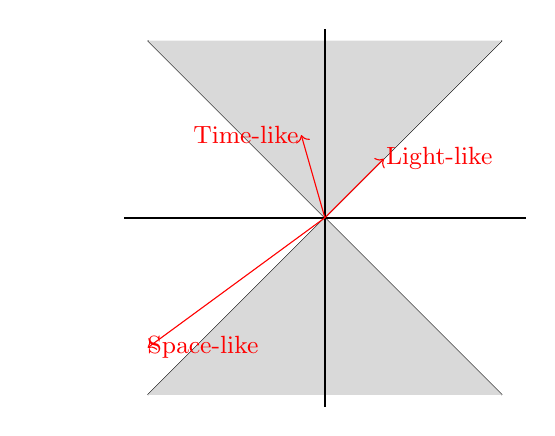
\begin{tikzpicture}[scale=1.5]
    \def\b{0.2} % semi-minor axis
    \pgfmathsetmacro{\h}{(1 + sqrt(1 + 4*\b^2)) / 2}
    \pgfmathsetmacro{\a}{sqrt(\h)}
    \draw (-1.5, -1.5) -- (1.5,  1.5);
    \draw (-1.5,  1.5) -- (1.5, -1.5);
    \fill[gray!30] (0,0) -- (1.5,1.5) -- (-1.5,1.5);
    \fill[gray!30] (0,0) -- (-1.5,-1.5) -- (1.5,-1.5);
    % \draw (0,  \h) ellipse [x radius = \a, y radius = \b];
    % \draw (0, -\h) ellipse [x radius = \a, y radius = \b];
    \draw [thick] (0,-1.6) -- (0,1.6);
    \draw [thick] (-1.7,0) -- (1.7,0);
    \draw [->, red] (0,0) -- (0.5,0.5) node {\hspace{4em}\small Light-like};
    \draw [->, red] (0,0) -- (-0.2,0.7) node {\hspace{-4em}\small Time-like};
    \draw [->, red] (0,0) -- (-1.5,-1.1) node {\hspace{4em}\small Space-like};
  \end{tikzpicture}
  \caption{The Light Cone}
\end{figure}
The gray shaded area is the accessible region of spacetime by light, the lightcone.

\subsection{Time Dilation}
Consider an object in frame $S$ moving with velocity $\vb{v}$, $\vb{s}\vdot\dd{\vb{x}}=\vb{v}\dd{t}$. Choose frame $S'$ to be ``co-moving'' with the object, so that the object is always at rest at the origin.

A small movement from event one to event two is:
\begin{align*}
  (\Delta s)^2&=(c\Delta t')^2\quad \text{in $S'$}\\
  &=(c\Delta t)^2-(\Delta x^2+\Delta y^2+\Delta z^2)\quad \text{in $S$}\\
\end{align*}
As an infinitesimal:
\begin{align*}
  (c\dd{t}')^2&=(c\dd{t})^2-(\dd{x}^2+\dd{y}^2+\dd{z}^2)\\
  &=\qty(c^2-v^2)\dd{t}^2
\end{align*}
So we define $t'$ in the $S'$ frame the proper time $\tau$, such that:
\begin{align*}
  \dd{t}'&\equiv\dd{\tau}=\sqrt{1-\frac{v^2}{c^2}}\equiv\sqrt{1-\beta^2}\\
  \beta&\equiv\frac{v}{c}
\end{align*}
Note that $\dd{\tau}\leq\dd{t}$, so \emph{moving clocks appear to run slow}
\begin{note}
  This is not an idle Observation. A large fraction of cosmic radiation at sea level comes from muons produced in pion decays in the upper atmosphere. THe muon lifetime of $\SI{2.2}{\micro\s}$ would imply that muons travelling at $c$ would only get $\sim\SI{600}{\m}$ if Galilean transformations are correct. Yet $~\frac12$ the muons produced at $\SI{2}{\km}$ make it to sea level (including losses from scattering). This means the muons were travelling at least at $\beta>0.976$ in our frame.
\end{note}

\subsection{Four-Vectors and Minkowski Space}
Express the coordinates for an event $(t,x,y,z)$ as a 4-dimensional vector:
\begin{align*}
  \vb{x}=\bmqty{ct\\x\\y\\z}=\bmqty{ct\\\vb{r}}
\end{align*}
In ordinary space (Euclidean): $\abs{\vb{x}}^2=c^2t^2+x^2+y^2+z^2$ (not what we want).

Define length in Minkowski space:
\begin{align*}
  \abs{\vb{x}}^2=\vb{x}\vdot\vb{x}=
  \vb{x}^T
  \underbrace{\bmqty{\dmat{1,-1,-1,-1}}}_{\text{``metric tensor'' }g}\vb{x}
  =c^2t^2-(x^2+y^2+z^2)
\end{align*}

The 4-dim space with metrix $g$ as above is called ``Minkowski space'',
``Euclidean space'' (flat space) has the identity $\id_{4\times4}$ as a metric. Special relativity says the length of a 4-vector in Minkowski space is the same in all inertial frame, i.e.\ invariant.

We began with the Galilean relationship between frames $S$ and $S'$. The real question is: What is the general form of the transformation between $S$ and $S'$ that conserves length in Minkowski space? \emph{Answer}: Homogeneous \emph{Lorentz Transformation}

Physics does not depend on (our definition of) absolute position or time. (This is a fundamental assumption of relativity).

Shifting the origin of $S$ must simply shift the origin of $S'$: $x\to x+a\implies x'\to x'+a$, so a transformation $L(x+a)=L(x)+a'$. Try $x=0$, $L(a)=L(0)+a'$, so $L(x+a)=L(x)+L(a)-L(0)$, define $L'(x)=L(x)-L(0)$ so that $L'(x+a)=L'(x)+L'(a)$, so $L(x)$ is a linear function of  $x$ plus a fixed offset.

Any linear transformation can be written sa a Poincare transformation $x'=Lx+a$; $L$ is a $4\times4$ matrix, $a$ translates the origin. Since physics is independent of where we place the origin, we only care about ``homogeneous Lorentz transformations'' (HLT) where we drop $a$.

\subsection{What do we know about $L$?}
We know $L$ must conserve 4-vector length\footnote{Note 4-vectors will be non-bolded from here on}:
\begin{align*}
  \abs{x}^2=x^T g x\iff \abs{x'}^2=(x')^T gx'=x^TL^TgLx
\end{align*}
So we need $\boxed{L^T gL=g}$.

If we consider components, $L_{ki}g_{kl}L_{lj}=g_{ij}$ forms 16 real equations, $g$ is symmetric, so there are $10$ constraints $\implies$ $\boxed{L\text{ has 6 d.o.f}}$ What are they?

Recall rotation matrices $A$ were defined by requiring conservation of length of the 3-vector in cartesian space:
\begin{align*}
  \abs{x}^2=\underbrace{c^2t^2}_{\text{untouched}}
  -\underbrace{\qty(x^2+y^2+z^2)}_{\text{conserved by }A}
  =\text{const.}
\end{align*}
So, rotations are a 3-D subset (subgroup) of an HLT.\@ $\therefore$ Euler angles are 3 of the d.o.f., what are the others?

Consider our frames $S$ and $S'$, were the origin of $S'$ is moving at constant velocity with respect to $S$: $x=v_xt,y=v_yt,z=v_zt$. We can always rotate $S$ and $S'$ so that the $x,x'$ are parallel to $\vb{v}$ (After all we just said rotations were a subset of HLT). Hence we can write the transformation as:
\begin{align*}
  \bmqty{ct'\\x'\\y'\\z'}=\bmqty{L_{00}&L_{01}\\L_{10}&L_{11}\\ &&1\\&&&1}
  \bmqty{ct\\x\\y\\z}
\end{align*}
Since $L$ satisfies $L^TgL=g$:
\begin{align*}
  L_{00}^2-L_{10}^2&=1\\
  L_{01}^2-L_{11}^2&=1\\
  L_{00}L_{01}-L_{10}L_{11}&=0
\end{align*}
The origin of $S'$ is $x'=0$, this means $0=L_{10}ct+L_{11}x$, which must satisfy $x=vt$, so $\beta\equiv\frac{v}{c}=-\frac{L_{10}}{L_{11}}$. Working out other combinations means:
\begin{align*}
  \bmqty{L_{00}&L_{01}\\L_{10}&L_{11}}=
  \bmqty{(\pm)\gamma&(\mp)\gamma\beta\\(\mp)\gamma\beta&(\pm)\gamma}
\end{align*}
Where the signs are arbitrary, and the lorentz factor $\gamma$ is:
\begin{align*}
  \gamma\equiv\frac1{\sqrt{1-\beta^2}}
\end{align*}
At low velocity ($\beta\to0$), we must recover the identity $L\to\smqty[\pm1\\&\pm1]$, so we choose the plus branch, hence we have:
\begin{align*}
  \boxed{L=\bmqty{\gamma&-\gamma\beta\\-\gamma\beta&\gamma\\&&1\\&&&1}}
\end{align*}
This is called a \emph{Lorentz boost along $x$}.

\begin{remark}
  Other solutions with different choices of $+$ and $-$ signs, such as:
  \begin{align*}
    L_{1}=\bmqty{\gamma&-\gamma\beta\\\gamma\beta&-\gamma}
    \quad\text{or}\quad
    L_{2}=\bmqty{-\gamma&\gamma\beta\\-\gamma\beta&\gamma}
  \end{align*}
  Represent reflections of the axes, $L_1$ represents a flip along the $x$ axis, or space inversion, and $L_2$ represents a flip along the $t$ axis, time reversal.

  These possibilities are not a part of \underline{continuous} Lorentz transformations, but could be interesting operators for other purposes.
\end{remark}

\subsection{General Boosts}
When the velocity between $S,S'$ is not along 1 axis, we can generalize with $\vb{r}_\|$ and $\vb{r}_\perp$, the parallel and perpendicular positions relative to the frame velocity $\vb{v}$, they are given by:
\begin{align*}
  \vb{r}_\|=\frac{(\vb{r}\vdot\bm{\beta})}{\beta^2}\bm{\beta}
  \qquad
  \vb{r}_\perp=\vb{r}-\vb{r}_\|
\end{align*}
So we have the following relationship between primed and unprimed variables:
\begin{align*}
  ct'&=\gamma ct-\gamma\beta\abs{\vb{r}_\|}=
  \gamma ct-\gamma(\vb{\bm{\beta}\vdot\vb{r}})\\
  \vb{r}'&=-\gamma\bm{\beta}ct+\gamma\vb{r}_\|+\bm{r}_\perp
  =-\gamma\bm{\beta}ct+\vb{r}+
  \frac{\gamma-1}{\beta^2}(\vb{r}\vdot\bm{\beta})\bm{\beta}  
\end{align*}
For a general $\beta$ we have:
\begin{align*}
  L_B=\bmqty{\gamma&-\gamma\bm{\beta}^T\\-\gamma\bm{\beta}
    &\id+(\gamma-1)\bm{\beta\beta}^T/\beta^2}
\end{align*}
In block matrix notation. Note that since $\beta$ has 3 components, these are our misisng 3 degrees of freedom.

A homogeneous Lorentz transform is a Boost and a rotation: $L_B L_A\equiv L$. A Poincare transform: $\vb{x}'\to L_BL_A\vb{x}+\vb{a}$, where $\vb{a}$ shifts origin.
\begin{note}
  We have the following properties of $L_B$ for boosts:
  \begin{enumerate}
  \item When $\beta\to0$, $L\to\id$
  \item $L_B^{-1}$ is formed by taking $\bm{\beta}\to-\bm{\beta}$
  \item $L_B$ is symmetric; $L_A=\smqty[\dmat{1,A}]$, $A$ antisymmetric; $L=L_BL_A$ is mixed.
  \end{enumerate}
\end{note}
\subsubsection{Addition of Velocities}
If $\bm{\beta}\|\bm{\beta}'$, define motion to be $x$-direction, we have:
\begin{align*}
  L'_BL_B=\bmqty{\gamma'&-\gamma'\beta'\\-\gamma'\beta'&\gamma'}
  \bmqty{\gamma&-\gamma\beta\\-\gamma\beta&\gamma}=
  \bmqty{\gamma'\gamma(1+\beta'\beta)&-\gamma'\gamma(\beta+\beta')\\
    -\gamma'\gamma(\beta+\beta')&\gamma'\gamma(1+\beta'\beta)}
\end{align*}
This is equivalent to \underline{one} transform $L_B''$ with:
\begin{align*}
  \beta''=\frac{\beta+\beta'}{1+\beta'\beta}
\end{align*}
With $\beta''<1$ still.

\textbf{Warning}: In general $L'_BL_B\neq L_BL'_B$, matrix is \underline{not} symmetric, so two proper Lorentz transforms (PLT) do \underline{not} add up to a PLT. \underline{But} two HLT \underline{do} add ip to a HLT (Call them $\Lambda$), in particulat, $L'_BL_B=L_B''L_A$, two PLTS add to a single PLT and a rotation.

\subsubsection{Lorentz Group}
The Lorentz group, $SO(3,1)$ HLT are orthogonal $4\times4$ matrices $O(4)$ with determinant $\det\Lambda=+1$, which means they are special $SO(4)$, and with the metric $\mathrm{diag}(1,-1,-1,-1)$, this is called $SO(3,1)$
\begin{note}[Group Structure of HLT]
  \begin{enumerate}
  \item Identity exists, $I=\id$
  \item Inverse exists, since $\Lambda^T\Lambda=\id$, $\Lambda^{-1}=\Lambda^T$
  \item Associative:
    \begin{align*}
      \Lambda_i(\Lambda_j\Lambda_k)=(\Lambda_i\Lambda_j)\Lambda_k
    \end{align*}
    This is always true for matrices.
  \item Closure: $\Lambda_1\Lambda_2=\Lambda_3$, subproof:
    \begin{align*}
      (\Lambda_1\Lambda_2)^T(\Lambda_1\Lambda_2)=
      \Lambda_2^T\Lambda_1^T\Lambda_1\Lambda_2=\id
    \end{align*}
    Hence $\Lambda_3$ is also HLT.
  \end{enumerate}
\end{note}

\subsection{Notation}
We note a 4-vector with greek indices, such as $x^\mu$, with $\mu=0,1,2,3$, the upper index means it is a contravariant vector, with indices:
\begin{align*}
  x^\mu=(ct,x^i)
\end{align*}
Where a roman index, such as $i$ denotes a 3-vector, with $i=1,2,3$

Under a Lorentz transform: $x^{\prime\mu}=\Lambda^\mu_\nu x^\nu$. We sum matched upper/lower greek indices (Einstein convention). The elements of $x^{\prime\mu}$ are:
\begin{align*}
  x^{\prime\mu}=(\gamma(x^0-\beta x^1),\gamma(x^1-\beta x^0),x^2,x^3)
\end{align*}
With the transform as before. Where did the lower index come from? The 1-Form (meaning 1 index) $x_\mu$ (lower Greek index) comes from $x^Tg$ ``covariant'' such that:
\begin{align*}
  x_\mu=(ct,-x^i)\equiv (ct,x_i)
\end{align*}
We ``lowered'' the index on $x$ by multiplying with the metric. What is the metric?
\begin{align*}
  g_{\mu\nu}=\vu{e}_\mu\vdot\vu{e}_\nu
\end{align*}
Given some basis, the vectors: $u$ and $v$, the product $u\vdot v=u^\mu\vu{e}_\mu\vdot v^\nu\vu{e}_\nu$

\begin{definition}[The Metric]
  The metric is a \emph{tensor} of rank 2 that contains the lengths and angles between basis vectors.
  \begin{itemize}
  \item In \emph{Minkowski} space, $g_{\mu\nu}$ is diagonal, but it is not a requirement.

    There is a corresponding tensor that ``raises'' indices, called the inverse metric $g^{\mu\nu}$
  \item In \emph{Minkowski} space, $g^{\mu\nu}$ has the same matrix form as $g_{\mu\nu}$, generally, $g^{\alpha\beta}g_{\beta\gamma}=\delta^{\alpha}_\gamma$
  \item The trace $g^{\alpha\alpha}=\delta^\gamma_\alpha\delta^\alpha_\gamma=4$ in 4 dimensions
  \end{itemize}
\end{definition}
We can formally move between upper and lower indices:
\begin{align*}
  x^\mu=g^{\mu\nu}x_\nu\qquad x_\mu=g_{\mu\nu}x^\nu
\end{align*}
\begin{note}
  Tensor notation, tensors are defined as having at least two indices, and are combinations of vectors via a tensor product:
  \begin{gather*}
    T^{\alpha\beta}=u^\alpha v^\beta\iff \bm{T}=u\otimes v\\
    T^{\alpha\beta\gamma}=u^\alpha v^\beta w^\gamma\iff \bm{T}=u\otimes v\otimes w
  \end{gather*}
  Where $\bm{T}$ is the tensor object.

  You can still freely move between upper and lower indices
  \begin{gather*}
    T_{\alpha\beta}=g_{\mu\alpha}g_{\nu\beta}T^{\mu\nu}\\
    T_\alpha^\beta=g_{\alpha\mu}T^{\mu\beta}
  \end{gather*}
  You just need a metric for each index you want to raise/lower
\end{note}
We can then see how each of the various objects transform under Lorentz transformations

\begin{itemize}
\item 1-form (vector) $x'_\mu=\Lambda^\mu_\nu x^\nu$
\item Tensor $T^{\prime\beta}_\alpha = \Lambda_\alpha^\gamma \Lambda_\delta^\beta T_\gamma^\delta$
\item Scalar $a'\vdot b'=\Lambda^\mu_\nu a^\nu\Lambda_\nu^\sigma b_\sigma=a^\nu b_\nu=a\vdot b$ which is invariant
  \begin{note}[Dot Product]
    Due to the metric of Minkowski space, the 4 vector dot product is:
    \begin{align*}
      a\vdot b\equiv a_\mu b^\mu=a^\mu b_\mu=a^0b^0-\vb{a\vdot b}
    \end{align*}
  \end{note}
\end{itemize}
We should now move onto a few physical quantities.

Imagine following the trajectory of a particle through 4-space. The trajectory will be $x^\mu(\lambda)$, where $\lambda$ is a parameter that monotonically varies along the curve. At any point $\lambda_0$ we may define a tangent 4-vector:
\begin{align*}
  \eta^\mu=\eval{\dv{x^\mu}{\lambda}}_{\lambda_0}
\end{align*}
For time-like particles, it is convenient to choose $\lambda=\tau$, the proper time:

\textbf{Proper Velocity}: $\bm{\eta}=\pdv{\vb{x}}{\tau}$ and thus the 4-velocity is: $\eta^\mu=\dv{x^\mu}{\tau}$.

If $S'$ is at rest with respect to a particle and moves with velocity $\vb{v}$ with respect to $S$, we have:
\begin{align*}
  x^\mu &= (ct,x^i) = (\gamma c\tau, \gamma v^i\tau)\\
  \eta^\mu &= (\gamma c, \gamma v^i)
\end{align*}
Notice that $\eta^2=\eta\vdot\eta=\gamma^2(c^2-v^2)=c^2$

Much more useful is the 4-momentum:
\begin{align*}
  p^\mu&=m\eta^\mu=(\gamma mc, \gamma mv^i)
\end{align*}
\begin{note}
  The components of the 4-momentum are useful to note, as the 3-vector components are just a boosted 3-momentum:
  \begin{align*}
    \vb{p}=m\gamma \vb{v}
  \end{align*}
  And the time component is related to the energy:
  \begin{align*}
    p^0=\frac{E}{c}=\gamma m c
  \end{align*}
\end{note}
The square of the 4-momentum is also useful:
\begin{align*}
  p^2=m^2c^2 = \qty(E/c)^2-(\vb{p\vdot p})
\end{align*}

\subsection{Conventions and ``Gotchas''}
\begin{enumerate}
\item In particle physics it is traditional to work in ``units of c''. The consstant speed of light is dimensionful and sets the natural scale of calculations. This means it is appropriate to define $\boxed{c=1}$. When units are required, we go back and put in however many $c$'s are required. Thus we have:

  $x^\mu\to(\tau,x^i)$ with $\tau$ in meters

  $p^\mu\to(E,\vb{p})$ with $E,m,\abs{\vb{p}}$ all in units of energy (eV)
\item \textbf{Metrics}: We have chosen $g_{\mu\nu}=\mathrm{diag}(1,-1,-1,-1)$, this is sensible as $p^2=E^2-\abs{\vb{p}}^2=m^2>0$
  \begin{enumerate}[label=\alph*)]
  \item Another choice often used in astrophysics is $g_{\mu\nu}=\mathrm{diag}(-1,1,1,1)$, then at $t=0$, $x^2=\abs{\vb{x}}^2$ However $p^2=-m^2<0$ which is technically valid but can be confusing.
  \item Also, sometimes (particularly in classical field theory), you need to stick with a Euclidean metric $\eta_{\mu\nu}=\mathrm{diag}(1,1,1,1)$, then some coordinates become \underline{complex}: $x^I=(ict,x^i)$
  \end{enumerate}
\item \textbf{Indices}: Some computer programs (you likely use) unfortunately chose to write 4-vectors as $x^{\tilde{\mu}}=(\vb{x},ct)$, with $\tilde{\mu}=1...4$. This was never necessary, and has led to many errors over the years.
\end{enumerate}
You have been warned.

\subsection{Relativistic Kinematics}
When we examine kinematics in the Newtonian ``classical'' limit, we invoke conservation laws. Consider a collision $A+B\to C+D$:
\begin{enumerate}
\item \underline{Mass} is conserved: $m_A+m_B=m_C+m_D$
\item \underline{Momentum} is conserved: $\vb{p}_A+\vb{p}_B=\vb{p}_C+\vb{p}_D$
\item \underline{Kinetic Energy}
  \begin{enumerate}[label=\alpha*)]
  \item decreases if collision is sticky $T_A+T_B>T_C+T_D$
  \item increases if collision is explosive $T_A+T_B<T_C+T_D$
  \item conserved if elastic $T_A+T_B=T_C+T_D$
  \end{enumerate}
\end{enumerate}

In relativistic kinematics, we assume all interactions are \emph{local}. (We will see why later -- it is in fact a very strong statement about the nature of the Universe, but it is also necessary for consistency.)

\begin{figure}[H]
  \centering
  \begin{tikzpicture}
    TODO
  \end{tikzpicture}
  \caption{Collision Picture}
\end{figure}

Our picture of collisions is 2 particles under free motion enter a ``black box'' in which they exchange a force, and then they travel off freely again.

\begin{enumerate}
\item \underline{Total Energy} is conserved
\item \underline{Momentum} is conserved
  \begin{enumerate}
  \item These are combined to give conservation of 4-momentum:
    \begin{align*}
      p^\mu_A+p^\mu_B=p^\mu_C+p^\mu_D
      \begin{cases}
        E_A+E_B=E_C+E_D\\
        \vb{p}_A+\vb{p}_B=\vb{p}_C+\vb{p}_D
      \end{cases}
    \end{align*}
  \end{enumerate}
\item \underline{Kinetic Energy}
    \begin{enumerate}[label=\alph*)]
  \item decreases if collision is sticky, \underline{mass} increases (particle creation)
  \item increases if collision is explosive, \underline{mass} decreases (particle decay, eg)
  \item conserved if elastic, so is mass
  \end{enumerate}
\end{enumerate}
We have given up conservation of mass, for conservation of energy

\begin{example}
  Two lumps of clay, each with mass $m$, collide head-on with speeds $\frac35c$. What is the final mass $M$ of the lump?
  \begin{align*}
    E_1+E_2&=E_M\\
    \vb{p}_1+\vb{p}_2&=\vb{p}_m=0
  \end{align*}
  Note we make a good choice of reference frame such that we end up in the rest frame of the final mass $M$, and the two lumps collide head on. Since $c=1$, we simply have $M=2E_m$, with $E_m$ given by:
  \begin{align*}
    E_m=\gamma m=\frac{m}{\sqrt{1-(3/5)^2}}=\frac54m
  \end{align*}
  Hence:
  \begin{align*}
    \boxed{M=\frac52m}
  \end{align*}
\end{example}
\begin{example}
  A particle of mass $M$ at rest decays into two particles of mass $m$. What is the \emph{speed} of each piece as it flies away?

  Speed is not a natural quantity (like $E$ or $p$), so we should find one of those and use:
  \begin{align*}
    \beta=\frac{\abs{\vb{p}}}{E}
  \end{align*}
  To derive the speed.

  So far we only have:
  \begin{align*}
    p^\mu&=p_1^\mu+p_2^\mu\\
    p^2&=M^2\\
    p_1^2=p_2^2=m^2
  \end{align*}
  To go further we should use \emph{invariants}
  \begin{enumerate}[label=\alph*)]
  \item Use $p^2=(p_1+p_2)^2$ and a convenient choice of reference frame such that:
    \begin{align*}
      p&=(M,0,0,0)\\
      p_{1/2}&=(E,0,0,\pm p_z)
    \end{align*}
    We can then expand the square of the sum:
    \begin{align*}
      p^2&=M^2\\
      (p_1+p_2)^2=m^2+m^2+2p_1\vdot p_2
    \end{align*}
    From our choice of frame, we can say:
    \begin{align*}
      p_1\vdot p_2&=E^2+\abs{\vb{p}}^2=2E^2-m^2\\
      \implies M^2&=2m^2+4E^2-2m^2=4E^2
    \end{align*}
    Thus we get:
    \begin{align*}
      E=\frac12M
    \end{align*}
    And for $\abs{\vb{p}}$:
    \begin{align*}
      \abs{\vb{p}}^2=E^2-m^2=\frac14M^2-m^2
    \end{align*}
    So the speed is:
    \begin{align*}
      \boxed{\beta=\sqrt{1-\frac{4m^2}{M^2}}}
    \end{align*}
  \end{enumerate}
\end{example}

\begin{example}
  A pion (135 MeV) decays to two photons. what are $E,\abs{\vb{p}},\beta$ of the photons?

  Using example 2.2:
  \begin{align*}
    E_\gamma&=\frac12M_\pi=67.5\text{MeV}\\
    \abs{\vb{p}_\gamma}^2&=E^2-\cancel{m^2}^0\\
    \implies\beta&=\frac{\vb{p}}{E}=\frac{E_\gamma}{E_\gamma}=1
  \end{align*}
  Good! It should travel at the speed of light

  So a \underline{massless} particle (like a photon), has a 4-momentum:
  \begin{align*}
    p^\mu=E(1,\vu{p})
  \end{align*}

  A \underline{massive} particle can also its 4-momentum written as:
  \begin{align*}
    p^\mu=E(1,\bm{\beta})
  \end{align*}
\end{example}

\begin{example}
  The Bevatron created antiprotons by hitting a fixed target (protons) with a beam of protons. The reaction is $p+p\to p+p+p+\bar{p}$. What was the threshold energy ($E_p^{\text{LAB}}$)

  The lab frame consists of a proton of energy $E$ hitting a stationary proton, and everything in the final state moves.

It is generally easier to work in the \underline{center of momentum} frame (where $\sum p^i=0$ or $\sum\vb{p}=0$), do not be sloppy in nomenclature, this is not center of mass.

In this frame, two particles collide head on and the 4 products are left at rest (at threshold). Using invariants:
\begin{align*}
  \underbrace{(p_1+p_2)^2}_{\text{frame inv.}}
  =(p_3+p_4+p_5+p_6)^2=16m^2
\end{align*}
The quantity above is frame invariant, so it is the same as in the lab frame:
\begin{align*}
  (p_1+p_2)^2_{\text{LAB}}=2m^2+2Em
\end{align*}
So equating these we have:
\begin{align*}
  16m^2=2m^2+2Em\implies E=7m
\end{align*}
This is the power of invariants!
\end{example}
\subsubsection{General Strategy}
\begin{enumerate}
\item Unless the solution is trivial, rewrite in terms of Lorentz scalars (invariants). Try to choose easy ones to evaluate.
\item Evaluate the scalars in \emph{any} frame --- the more straight forward the better.
\item If you need a particular quantity, e.g. $\beta$ of a certain particle, consider regrouping momenta before squaring
\end{enumerate}

\subsection{Mandelstam Invariants}
For the general process $A+B\to C+D$, the following quantities are named:
\begin{align*}
  s\equiv(p_A+p_B)^2&=(p_C+p_D)^2\\
  t\equiv(p_A-p_C)^2&=(p_D-p_B)^2\\
  u\equiv(p_A-p_D)^2&=(p_C-p_B)^2
\end{align*}
If we sum them we get a fairly useful quantity:
\begin{align*}
  s+t+u=m_A^2+m_B^2+m_C^2+m_D^2
\end{align*}
Returning to $pp\to ppp\bar{p}$, we used the invariant $s$ to calculate everything

% -*- TeX-master: "master.tex" -*-
\newcommand{\up}{\uparrow}
\newcommand{\dn}{\downarrow}
\section{Symmetry}
The study of symmetry has been a central theme in the study of physics. In 1917 Emmy Noether proved that (for a specific type of field-complex, 4-dimensional) a symmetry of the Hamiltonian implied the existence of a conserved quantity

You have studied the correspondence of symmetries and conserved quantities in classical and quantum mechanics:
\begin{itemize}
\item Time translation invariance $\iff$ Energy conservation
\item Space translation invariance $\iff$ Momentum conservation
\item Rotational invariance $\iff$ Angular momentum conservation
\end{itemize}

The construction of the Standard Model (and much of theoretical thought) has been largely the identification of the symmetries associated with observed conserved quantities.

\begin{aside}
  Not all conserved quantities must come from symmetries, e.g.\ solitons and other topological properties etc.
\end{aside}

A conserved quantity is one that is unchanged by a transformation, e.g.\ a Lorentz scalar under a Lorentz transformation.

The set of possible transformations of a given type have the properties of a \underline{group}. Hence, we study groups and algebras

\subsection{Group Theory}
Reminder of group definitions
\begin{enumerate}
\item Clousure: if $A\in G$, $B\in G$, then $AB\in G$
\item $\exists$ an identity: $I\in G$
\item Every element has an inverse: $A\in G$, $AA^{-1}=A^{-1}A=I$ with $A^{-1}\in G$
\item Associativity: $(AB)C=A(BC)$
\end{enumerate}

\subsubsection{Rotation Group}
Consider rotation by angle $\theta$ about the $z$-axis:
\begin{align*}
  \pmqty{x'\\y'\\z'}=
  \underbrace{\pmqty{\cos\theta & \sin\theta&\\
      -\sin\theta&\cos\theta&\\&&1}}_{R_z(\theta)}
  \pmqty{x\\y\\z}
\end{align*}
Similarly:
\begin{align*}
  R_x(\theta)=
  \pmqty{1\\&\cos\theta&\sin\theta\\&-\sin\theta&\cos\theta}
  \qquad
  R_y(\theta)=
  \pmqty{\cos\theta&&\sin\theta\\&1&\\-\sin\theta&&\cos\theta}
\end{align*}
Two successive rotations is also a rotation (closure). Can you quickly show the other group requirements?

Rotations leave the length of a vector invariant:
\begin{align*}
  {(x')}^2=x_i'x_i'=R_{ij}R_{ik}x_j x_k
  ={(R^T)}_{ji}R_{ik}x_j x_k=\delta_{jk}x_j x_k
  =x_k x_k=x^2
\end{align*}

So rotations form a three-dimensional orthogonal group, called $SO(3)$. In addition:
\begin{align*}
  \det{R}=\cos^2\theta+\sin^2\theta=1
\end{align*}
So the rotation group is $SO(3)$, S for special, O for orthogonal.

Recal the Lorentz group is $SO(3,1)$. Rotations are a \underline{subgroup} of the Lorentz Group:
\begin{align*}
  \Lambda^\mu_\nu=\pmqty{\text{Boosts}&\\&3\times3\text{ Rotations}}
\end{align*}
So the Lorentz group $=$ Boosts + Rotations

\subsubsection{Spin}
Consider a particle of mass $m$ at rest. Its four-momentum is:
\begin{align*}
  p^\mu=\pmqty{m\\0\\0\\0}
\end{align*}
Certainly the particle's four-momentum is invariant under rotations. The spin of the particle tells you how the wavefunction of the particle transforms  under the rotation group:
\begin{itemize}
\item Spin 0: $R=\bm{1}$ Trivial
\item Spin $\frac12$: $R_i=\exp{i\frac12\theta_i\sigma_i}$ where $\sigma_i$ are the Pauli matrices $(2\times2)$
\item Spin 1: $R=3\times3$ Rotation matrices (see above)
\item Spin $\frac32$: $R=4\times4$ matrices
\item Spin $j$: $R=(2j+1)\times(2j+1)$ matrices
\end{itemize}
So the spin of a particle is related to its \underline{representation} of the rotation group

Formally, a representation is a homomorphic mapping of a group onto the matrices $(GL_n)$ of rank $n$.

The symmetry associated with rotations is continuous. Hence, rather than work directly with the rotation matrices, we may work with the significantly simpler infinitesimal roations:

Let $R(\theta)=\exp{i\theta_i T_i}\equiv e^{i\theta_i T_i}$, where $T_i$ are matrices, $i=x,y,z$, and $\exp$ of a matrix is just the shorthand for:
\begin{align*}
  \exp{M}=e^M\equiv\sum_{i=0}^\infty\frac{M^n}{n!}
\end{align*}
We know that $R^TR\equiv\bm{1}$, so that $\exp{i\theta_iT_i}^T\exp{i\theta_iT_i}=\bm{1}$. Consider $\theta_i$ to be infinitesimal and expand:
\begin{align*}
  (\bm{1}+i\theta_iT_i^T+\cdots)
  (\bm{1}+i\theta_iT_i^T+\cdots)&=\bm{1}\\
  \implies \theta_i\qty[T_i^T+T_i]&=0
\end{align*}
Thus we arrive at $T_i^T=-T_i$, that is, $T_i$ are \underline{antisymmetric matrices}.

Consider: $R_x(\theta)$ with $\theta\ll 1$:
\begin{align*}
  R_x(\theta\ll1)&=\pmqty{1\\&1&-\theta\\&\theta&1}\\
  &=\bm{1}+\theta\pmqty{0&0&0\\0&0&-1\\0&1&0}
\end{align*}
From above, we can then identify $iT_x$ as this second matrix. Repeating the above process for $R_y,R_z$, we obtain a full set of generators of $SO(3)$:
\begin{align*}
  iT_x=\pmqty{0&0&0\\0&0&-1\\0&1&0}\quad
  iT_y=\pmqty{0&0&-1\\0&0&0\\1&0&0}\quad
  iT_z=\pmqty{0&-1&0\\1&0&0\\0&0&0}
\end{align*}

Consider two successive rotations:
\begin{gather*}
  R(\theta)R(\theta')=R(\theta'')\\
  R(\theta)=\bm{1}+i\theta\vdot T
\end{gather*}
Since they form a group, the right hand side should also be a rotation, and we have our definition of the generator below, with $\theta\vdot T=\theta_iT_i$. Plugging this form into the above:
\begin{align*}
  (\bm{1}+i\theta\vdot T+\frac12(i\theta\vdot T)^2+\cdots)
  (\bm{1}+i\theta'\vdot T+\frac12(i\theta'\vdot T)^2+\cdots)=
  (\bm{1}+i\theta''\vdot T+\frac12(i\theta''\vdot T)^2+\cdots)
\end{align*}
This gives you that $\theta+\theta'=\theta''$ to first order, $\order{\theta}$. If we go to second order, we would find that $\theta+\theta'=\theta''+\alpha$ where $\alpha\sim\order{\theta^2}$. Here we find that:
\begin{align*}
  -\frac12\qty[(\theta\vdot T)^2+(\theta'\vdot T)^2+2(\theta\vdot T)(\theta'\vdot T)]=-\frac12\qty[(\theta''\vdot T)^2-2i\alpha\vdot T]
\end{align*}
Now the second order term will tell us:
\begin{align*}
  (\theta''\vdot T)^2=\qty[\theta\vdot T+\theta'\vdot T-\alpha\vdot T]^2
\end{align*}
However we can essentially ignore the $\alpha\vdot T$ cross terms since all the other terms are at least order $\theta$, and the resulting multiplied term would be $\order{\theta^3}$ or greater, which we do not need to consider. Hence we find:
\begin{align*}
  (\theta''\vdot T)^2=(\theta\vdot T)^2+(\theta'\vdot T)^2+(\theta'\vdot T)(\theta\vdot T)+(\theta\vdot T)(\theta'\vdot T)
\end{align*}
This gives a relation between $\alpha$ and the other second order terms:
\begin{align*}
  -2i\alpha\vdot T=
  (\theta\vdot T)(\theta'\vdot T)-(\theta'\vdot T)(\theta\vdot T)
\end{align*}
Since $\alpha\sim\order{\theta^2}$, and for the above equation to hold it must be proportional to $\theta\theta'$. Let $\alpha_i\equiv-\frac12f_{jki}\theta_jtheta'_k$. We then find:
\begin{align*}
  if_{jki}\theta_j\theta'_kT_i&=\theta_j\theta'_k\qty[T_jT_k-T_kT_j]\\
  \implies if_{jki}T_i=T_jT_k-T_kT_j
\end{align*}
Define the commutator: $\comm{A}{B}\equiv AB-BA$, so that we can relabel:
\begin{align*}
  \boxed{\comm{T_i}{T_j}=if_{ijk}T_k}
\end{align*}
From this we find $f_{ijk}=-f_{jik}$. These are called structure constants, and are real valued.

This commutator above tells us that $SO(3)$ is a \underline{Lie Group}, i.e. a continuous group (on a differentiable manifold).

The generators $T_i$ of $SO(3)$ form a \underline{graded Lie algebra} with structure constants $f_{ijk}$

The structure constants for $SO(3)$ are $f_{ijk}=\veps_{ijk}$, with $\veps_{123}=+1$, the totally antisymmetric tensor. In other words the commutators are given as:
\begin{align*}
  \comm{T_x}{T_y}&=iT_z\\
  \comm{T_y}{T_z}&=iT_x\\
  \comm{T_z}{T_x}&=iT_y
\end{align*}

A \underline{representation} of the $SO(3)$ Lie algebra is any set of matrices which satisfy
\begin{align*}
  \comm{T_i}{T_j}=i\veps_{ijk}T_k
\end{align*}
The $3\times 3$ matrices we have written are called the \underline{fundamental representation} (also known as the \underline{defining representation}).

Recal this was associated with spin-1 particles.

\subsection{Spin $\frac12$ Representation}
The generators associated with spin-$\frac12$ are:
\begin{align*}
  T_x=\frac12\pmqty{&1\\1&}\quad
  T_y=\frac12\pmqty{&i\\-i&}\quad
  T_z=\frac12\pmqty{1& \\ &-1}
\end{align*}
Which are related to the Pauli Matrices, i.e. $T_i=\frac12\sigma_i$.

One can show that these $2\times 2$ matrices $T_i$ satisfy $\comm{T_i}{T_j}=i\veps_{ijk}T_k$, so they do form a representation of $SO(3)$.

The $T_i$ for this representation are \underline{not} antisymmetric, but they are Hermitian:
\begin{align*}
  T_i^\dag=T_i
\end{align*}
The rotation matrices $R=\exp{iT}$ are therefore \underline{unitary}:
\begin{align*}
  R^\dag R=(e^{iT})^\dag e^{iT}=e^{-iT^\dag}e^{iT}=e^{-iT}e^{iT}=\bm{1}
\end{align*}
To emphasize this, let's call these $2\times2$ matrices $U$ instead of $R$, so:
\begin{align*}
  U^\dag U=\bm{1}
\end{align*}

These $2\times2$ complex, unitary rotation matrices represent the group $SO(3)$, \underline{but} they also represent the group $SU(2)$, where $SU(2)$ means \textbf{s}pecial (determinant 1) \textbf{u}nitary $\mathbf{2\times2}$ matrices.
\begin{aside}
  Note that $\det U$ can be shown to be $1$:
  \begin{align*}
    \det U=\det e^{iT}=\exp{i\Tr[T]}=e^{i0}=1
  \end{align*}
  Since $T$ are traceless in general.
\end{aside}

So we have proven the groups $SU(2)$ and $SO(3)$ have the \underline{same} Lie algebra. Thus the groups are identical as far as ``small'' rotations are concerned:
\begin{align*}
  SU(2)\underbrace{\approxeq}_{\text{Isomorphic}} SO(3)
\end{align*}

While the $3\times3$ $SO(3)$ matrices act on ordinary space $(x,y,z)$, the $2\times2$ complex $SU(2)$ matrices act on a complex, 2-dimensional ``spin'' space. We call this the \underline{fundamental} representation of $SU(2)$, but the \underline{spinor} representation of $SO(3)$.
\begin{remark}
  The so-called \underline{Classical Lie Groups} are $SO(n+1)$, $SU(n)$, and $SP(n+1)$, with the $p$ for symplectic. Some exceptions to these are $G_2, F_4, E_6, E_7, E_8$.

  It is also important to note that $SO(2)\approxeq U(1)$, so 2D rotations are equivalent to unitary numbers $e^{i\theta}$
\end{remark}

\subsection{Isospin}
Isospin (or Isotropic spin) is the symmetry of the strong interaction (QCD):
\begin{figure}[H]
  \centering
  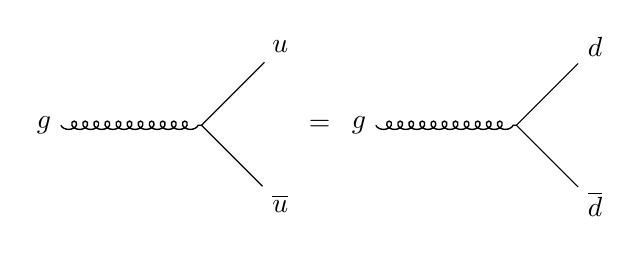
\begin{tikzpicture}[scale=2.0]
    \begin{feynhand}
      % vertices
      \vertex (p11) at (1.5,0.5) {$u$};
      \vertex (p12) at (1.5,-0.5) {$\bar{u}$};
      \vertex (a1) at (0,0) {$g$};
      \vertex (b1) at (1,0);
      % propagators
      \propag [gluon] (a1) to (b1);
      \propag (b1) to (p11);
      \propag (b1) to (p12);
      \vertex (eq) at (1.75,0) {=};
      % vertices
      \vertex (p21) at (3.5,0.5) {$d$};
      \vertex (p22) at (3.5,-0.5) {$\bar{d}$};
      \vertex (a2) at (2,0) {$g$};
      \vertex (b2) at (3,0);
      % propagators
      \propag [gluon] (a2) to (b2);
      \propag (b2) to (p21);
      \propag (b2) to (p22);
    \end{feynhand}
  \end{tikzpicture}
  \caption{Isospin Conservation in QCD}
  \label{fig:isospin}
\end{figure}
So in QCD, $u$ and $d$ are interchangeable. This is the reason for isospin.

But, recall that $m_u\neq m_d$. So how is it possible that we can interchange $u$ and $d$?
\begin{figure}[H]
  \centering
  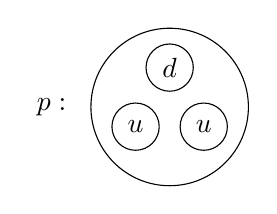
\begin{tikzpicture}
    \node at (0,0) {$p:$};
    \draw (1.500, 0.00) circle (1.0);
    \draw (1.500, 0.50) circle (0.3) node {$d$};
    \draw (1.067,-0.25) circle (0.3) node {$u$};
    \draw (1.933,-0.25) circle (0.3) node {$u$};
  \end{tikzpicture}
  \caption{Proton representation}
  \label{fig:proton}
\end{figure}
Recall the structure of the proton, and that $m_p\gg m_u,m_d$, this is because the proton mass is ``dynamical'' and is not due to the quark masses. So isospin is a good symmetry due to this difference in proton and up/down masses.

In group theory terms, we say that $\pmqty{u\\d}$ transform as a doublet under $SU(2)$ isospin

\begin{remark}
  \underline{\textbf{WARNING}}: $SU(2)$ ``isospin'' has nothing to do with $SU(2)$ spin! The mathematics is the same, but the physics is entirely different!
\end{remark}
One consequence of isospin is that $m_p=m_n$, this means that $\pmqty{p\\n}$ transform as an isospin doublet:
\begin{figure}[H]
  \centering
  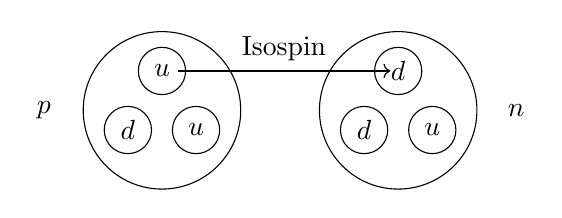
\begin{tikzpicture}
    \node at (0,0) {$p$};
    \draw (1.500, 0.00) circle (1.0);
    \draw (1.500, 0.50) circle (0.3) node {$u$};
    \draw (1.067,-0.25) circle (0.3) node {$d$};
    \draw (1.933,-0.25) circle (0.3) node {$u$};
    \node at (6,0) {$n$};
    \draw (4.500, 0.00) circle (1.0);
    \draw (4.500, 0.50) circle (0.3) node {$d$};
    \draw (4.067,-0.25) circle (0.3) node {$d$};
    \draw (4.933,-0.25) circle (0.3) node {$u$};
    \draw[->] (1.700, 0.500) -- (4.400, 0.500);
    \node at  (3.050, 0.500) [above] {Isospin};
  \end{tikzpicture}
  \caption{Proton \& Neutron in Isospin}
  \label{fig:isospinpn}
\end{figure}
Historically, this was the motivation for Heisenberg to suggest isospin differentiated ``nucleons,'' like $s_z=\pm\frac12$ differentiates the degeneracy in spin $\frac12$ systems.
\begin{note}
  The nuclear physicists use the much better term ``isobaric'' spin.

  E.g., Mirror nuclei, like $^7_3$Li/$^7_4$Be and $^{11}_5$B/$^{11}_6$C have nearly identical binding energies (after correcting for coulomb interaction)
\end{note}

\begin{definition}[Antiquarks]
  The so called antiquarks $\bar{u}$ and $\bar{d}$ are simply defined to be the complex conjugate of $u,d$.

  In group theory, this corresponds to $T_i$ representating the same algebra as $-T_i^*$:
  \begin{align*}
    \comm{T_i}{T_j}&=if_{ijk}T_k\\
    \comm{T_i^*}{T_j^*}&=-if_{ijk}T_k^*\\
    \implies\comm{(-T_i^*)}{(-T_j^*)}&=if_{ijk}(-T_k^*)
  \end{align*}
\end{definition}

For $SU(2)$, the complex conjugate representation is unitarily equivalent to the original representation:
\begin{align*}
  \underbrace{\pmqty{&-1\\1}}_{U}\qty(-T_i^*)
  \underbrace{\pmqty{&1\\-1}}_{U^\dag}=T_i
\end{align*}
For $T_i$ in the spin $\frac12$ representation, the representation is \underline{pseudoreal}.

Antiquarks transform as the c.c. rep., called the $\bar{2}$ representation:
\begin{align*}
  -T_i^*\pmqty{\bar{u}\\\bar{d}}&=\pmqty{\bar{u}'\\\bar{d}'}\\
  T_i\pmqty{-\bar{d}\\\bar{u}}&=\pmqty{-\bar{d}\\\bar{u}}
\end{align*}
Therefore, we can say that instead of using complex conjugate versions of the same algebra, we can use the usual spin-$\frac12$, instead on $\pmqty{-\bar{d}\\\bar{u}}$
\begin{definition}[Pions]
  Pions (or more generally mesons) are pairs of $q\bar{q}$, quarks and antiquarks.
\end{definition}
The strong interaction (QCD) not only binds quarks into $p,n$, it also binds quarks with antiquarks into \underline{pions}.

\begin{figure}[H]
  \centering
  
  \caption{Pion definition}
  \label{fig:pion}
\end{figure}
The charge of the pion is given by the sum of the charges of the $u$ and $\bar{d}$ quarks, that is $+\frac23+\frac13=1$.

In particular, pions are formed from the product of $\pmqty{u\\d}$ and $\pmqty{-\bar{d}\\u}$ isospin doublets. These are combined in the same way that we add spins:
\begin{example}[Adding Spins]
  Adding 2 spin-$\frac12$ particles, we have the following:
  \begin{align*}
    &\ket{J,J_z}\\
    &\ket{1, 1}=\ket{\up\up}\\
    &\ket{1, 0}
    =\frac1{\sqrt{2}}\qty(\ket{\up\dn}+\ket{\dn\up})\\
    &\ket{1,-1}=\ket{\dn\dn}\\
    &\ket{0,0}
    =\frac1{\sqrt{2}}\qty(\ket{\up\dn}-\ket{\dn\up})
  \end{align*}
  The first 3 are the spin 1 triplet, and the last 1 is the spin 0 singlet
\end{example}
\begin{example}[Adding IsoSpins]
  The math is exactly the same, except instead of $\up/\dn$ we will have $u,\bar{u},d,-\bar{d}$
  \begin{align*}
    &\ket{I,I_3}\\
    &\ket{1, 1}=\ket{u(-\bar{d})}\equiv\pi^+\\
    &\ket{1, 0}=\frac1{\sqrt{2}}\qty(\ket{u\bar{u}+d(-\bar{d})})\equiv\pi^0\\
    &\ket{1,-1}=\ket{d\bar{u}}\equiv\pi^-\\
    &\ket{0,0}=\frac1{\sqrt{2}}\qty(\ket{u\bar{u}-d(-\bar{d})})\equiv???
  \end{align*}
  The first 3 are the isospin 1 triplet, the pions, and the last is different, we will come back to it
\end{example}
So, we have isospin doublets of $\pmqty{p\\n}$ and $\pmqty{-n\\p}$, and the isospin triplet of $\pmqty{\pi^+\\\pi^0\\\pi^-}$. The pion masses are:
\begin{align*}
  m_{\pi^\pm}&=\SI{139.56}{\mega\eV}\\
  m_{\pi^0}&=\SI{134.97}{\mega\eV}
\end{align*}
\begin{note}
  Isospin is \underline{not} a symmetry of the electromagnetic interaction, that is:
  \begin{figure}[H]
  \centering
  \begin{tikzpicture}[scale=2.0]
    \begin{feynhand}
      % vertices
      \vertex (p11) at (1.5,0.5) {$u$};
      \vertex (p12) at (1.5,-0.5) {$\bar{u}$};
      \vertex (a1) at (0,0) {$\gamma$};
      \vertex (b1) at (1,0);
      % propagators
      \propag [gluon] (a1) to (b1);
      \propag (b1) to (p11);
      \propag (b1) to (p12);
      \vertex (eq) at (1.75,0) {$\neq$};
      % vertices
      \vertex (p21) at (3.5,0.5) {$d$};
      \vertex (p22) at (3.5,-0.5) {$\bar{d}$};
      \vertex (a2) at (2,0) {$\gamma$};
      \vertex (b2) at (3,0);
      % propagators
      \propag [gluon] (a2) to (b2);
      \propag (b2) to (p21);
      \propag (b2) to (p22);
    \end{feynhand}
  \end{tikzpicture}
  \caption{QED does \underline{not} care about isospin}
  \label{fig:isospin}
\end{figure}
This is because the electromagnetic charge of $u$ and $d$ are not equal, $Q_u=+\frac23$ and $Q_d=-\frac13$
\end{note}
Isospin has \underline{dynamical} implications. Consider $\pi N$ ($N=n,p$), that is $\pi N\to\pi'N'$. Since $\pi$ has $I=1$ and $N$ has $I=\frac12$, the state $(\pi N)$ can have $I=\frac12,\frac32$. Since $I$ is conserved, all $\pi N$ scattering processes can be reduced to just $2$ amplitudes.

\begin{example}[$\pi^+p\to\pi^+p$]
  Isospin: $\ket{\frac32,\frac32}\to\ket{\frac32,\frac32}$.

  The reaction is pure in isospin, so $A(\pi^+p\to\pi^+p)\equiv A_{3/2}$
\end{example}
Next consider a mixed process:
\begin{example}[$\pi^-p\to\pi^-p$]
  Isospin: We are adding $\ket{1,-1}$ to $\ket{\frac12,\frac12}$:
  \begin{align*}
    \ket{1,-1}\oplus\ket{\frac12,\frac12}
    =\frac1{\sqrt{3}}\ket{\frac32,-\frac12}
    -\sqrt{\frac23}\ket{\frac12,-\frac12}
  \end{align*}
  The reaction is no longer pure in isospin, but the amplitude would be the square of the coefficients: so $A(\pi^-p\to\pi^-p)= \frac13A_{3/2}+\frac23A_{1/2}$
\end{example}
The takeaway from this is that all ten $\pi N$ scattering amplitudes can be expressed in terms of $A_{3/2}$ and $A_{1/2}$.

Isospin conservation also imposes important constraints on string interaction processes.

\begin{example}[$d+d\to \,^4\text{He}+\pi^0$]
  Since the deuteron $d$ is a combination of $p\oplus n$, $I=0$, a similar argument shows $I=0$ for $^4\text{He}$, but $\pi^0$ has $I=1$. Hence this process would violate isospin conservation, and can only occur electromagnetically. It was only in the mid-2000's that experimenters at Indiana University claimed a detection of this rare process.
\end{example}

\begin{example}
  The branching fraction (\% of decays that occur in a given channel) for $\psi'\to J/\psi+\pi^0+\pi^0$ is $\sim20\%$, while $\psi'\to J/\psi+\pi^0$ is only $\sim0.1\%$. The $\psi'$ and $J/\psi$ are $c\bar{c}$ bound states ($I=0$), and again, the decay to one pion is inhibited, while the decay to two pions is not.
\end{example}

\begin{definition}{$\rho$ meson}
  The pions have spin $0$, the quark and antiquark have opposite spin:
  \begin{align*}
    \ket{\pi^+}=\ket{u(-\bar{d})}\otimes\underbrace{\frac1{\sqrt{2}}
      \qty(\ket{\up\dn-\dn\up})}
    _{\ket{0,0}\text{ state}}
  \end{align*}
  There is also a state with aligned spins:
  \begin{align*}
    \ket{\rho^+}=\ket{u(-\bar{d})}\otimes
    \begin{cases}
      \ket{\up\up} & =\ket{1,1} \\
      \frac1{\sqrt{2}}\ket{\up\dn+\dn\up}
      & =\ket{1,0} \\
      \ket{\dn\dn} & =\ket{1,-1}
    \end{cases}
  \end{align*}
\end{definition}
The $\rho$ (``rho'') is a spin-1 particle and an isospin triplet (like the pion):
\begin{align*}
  \pmqty{\rho^+\\\rho^0\\\rho^-}\text{ Isospin triplet}\quad
  m_{\rho^\pm}\approx m_{\rho^0}\equiv m_{\rho}\approx\SI{770}{\MeV}
\end{align*}

\begin{definition}{$\omega$ meson}
  This is the $I=0$ version of the $\rho$:
  \begin{align*}
    \ket{\omega}=\frac1{\sqrt{2}}\qty(\ket{u\bar{u}}+\ket{d(-\bar{d})})
    \otimes
    \begin{cases}
      \ket{\up\up} & =\ket{1,1} \\
      \frac1{\sqrt{2}}\ket{\up\dn+\dn\up}
      & =\ket{1,0} \\
      \ket{\dn\dn} & =\ket{1,-1}
    \end{cases}
  \end{align*}
\end{definition}
The $\omega$ is a singlet and has mass $m_\omega=\SI{783}{\MeV}\approx m_\rho$, this is NOT a consequence of isospin.

We will return to $I=0$ version of the pion later.

\subsection{Nomenclature}
\begin{definition}[Hadron]
  A hadron is a particle composed of quarks and/or antiquarks:
  \begin{enumerate}[label=(\alph*)]
  \item \underline{Mesons}: $q\bar{q}$ pairs like $\pi,\rho,\omega$
  \item \underline{Baryons}: $qqq$ states like $p,n$,

    Antibaryons are $\bar{q}\bar{q}\bar{q}$ states
  \end{enumerate}
\end{definition}

\begin{definition}[$\Delta$ baryon]
  This is the $I=\frac32$, $J=\frac32$ version of the proton:
  \begin{align*}
    \Delta^{++}&=``uuu''\\
    \Delta^{+ }&=``uud''\\
    \Delta^{0 }&=``udd''\\
    \Delta^{- }&=``ddd''
  \end{align*}
  With mass $m_\Delta=\SI{1232}{\MeV}$, we will write these more carefully in a moment.
\end{definition}
Consider the $\Delta^{++}$ with $J_z=+\frac32$, this is the state $\ket{\Delta^{++},J_z=+\frac32}=\ket{uuu}\otimes\ket{\up\up\up}$
This state is totally symmetric under the interchange of any pair of quarks. But the Pauli statistics that govern fermions insist this must be antisymmetric!

The solution? Color. We now write the state as $\ket{\Delta^{++},J_z=+\frac32}=\frac1{\sqrt{6}}\veps_{ijk}\ket{uuu}\otimes\ket{\up\up\up}$, where $i=1,2,3$ are the 3 ``colors'' red, green, blue. Thus we have totally symmetric \underline{quark} and \underline{spin} states, but an antiymmetric \underline{color} state, with a general state of
\begin{align*}
  \psi=\psi(\text{space})\otimes
  \psi(\text{flavor})\otimes
  \psi(\text{spin})\otimes
  \psi(\text{color})
\end{align*}
So the $\Delta$ states have ``flavor'' structure of:
\begin{align*}
  \Delta^{++}&=\ket{uuu}\\
  \Delta^{+ }&=\frac1{\sqrt{3}}\ket{uud+udu+duu}\\
  \Delta^{0 }&=\frac1{\sqrt{3}}\ket{udd+dud+ddu}\\
  \Delta^{- }&=\ket{ddd}
\end{align*}
With the color indices and spin states suppressed.

\textbf{Question}: The proton has $J=\frac12$. Is there are $\ket{uuu}$ state with $J=\frac12$? No, only $J=\frac32$ has a completely symmetric spin of three spin-$\frac12$ quarks

\subsection{Proton and Neutron}
$p,n,$ and $\Delta$ are all constructed from three $I=\frac12$ doublets:
\begin{align*}
  \pmqty{u\\d}\otimes\pmqty{u\\d}=
  \begin{cases}
    uu \\ \frac1{\sqrt{2}}(ud+du) \\ dd \\
    \frac1{\sqrt{2}}(ud-du)
  \end{cases}
\end{align*}
With the first 3 being isospin 1 and the last isospin 0.

In the language of group theory, this is:
\begin{align*}
  \underbrace{2}_{\text{doublet}}\otimes 2 = \underbrace{3}_{\text{triplet}}
  \oplus \underbrace{1}_{\text{singlet}}
\end{align*}
Let's add the third quark:
\begin{align*}
  \pmqty{u\\d}\otimes
  \pmqty{uu\\\frac1{\sqrt{2}}(ud+du)\\dd}
  =\pmqty{uuu\\\frac1{\sqrt{3}}duu+\sqrt{\frac23}u\frac1{\sqrt{2}}(ud+du)\\
    \frac1{\sqrt{3}}udd+\sqrt{\frac23}d\frac1{\sqrt{2}}(ud+du)\\ ddd}
  \oplus \pmqty{\sqrt{\frac23}duu-\frac1{\sqrt{6}}u(ud+du)\\
  \frac1{\sqrt{6}}d(ud+du)-\sqrt{\frac23}udd}
\end{align*}
Or $2\otimes3=4\oplus2$, The 4 is clearly the $\Delta$, but the doublet is NOT the $p,n$ doublet, since it is not symmetric in exchange of the first 2 quarks.

Of course there is also the state from $2\otimes 1$:
\begin{align*}
  \pmqty{u\\d}\otimes\frac1{\sqrt{2}}\qty(ud-du)=
  \begin{cases}
    \frac{1}{\sqrt{2}}u(ud-du)\\
    \frac{1}{\sqrt{2}}d(ud-du)
  \end{cases}
\end{align*}
Which is antisymmetric in the last two quarks.

Group theory: $2\otimes2\otimes2=2\otimes(3\oplus1)=4\oplus2_S\oplus2_A$, where $S,A$ mean symmetric/antisymmetric in the last 2 quarks.

To build $p,n$, we need to combine isospin with spin to make a totally symmetric state. Color will then make it antisymmetric as before.

We've shown spin and isospin share the same mathematics. Let's use that property. For spin, we also get $2\otimes2\otimes2=4\oplus2_S\oplus2_A$. So $\Delta=(4,4)$, where the first is isospin and the second is spin. This means that $p,n=(2_S,2_S)\oplus(2_A,2_A)$.

So to construct $p$ with $J_z=+\frac12$:
\begin{align*}
  \qty[\sqrt{\frac23}duu-\frac1{\sqrt{6}}u(ud+du)]\otimes
  \qty[\sqrt{\frac23}\dn\up\up-\frac1{\sqrt{6}}\up(\up\dn+\dn\up)]\oplus
  \qty[\frac1{\sqrt{2}}u(ud-du)]\otimes
  \qty[\frac1{\sqrt{2}}\up(\up\dn-\dn\up)]\\
  \equiv duu\qty[\frac23\dn\up\up-\frac13\up\up\dn-\frac13\up\dn\up]
  uud\qty[-\frac13\dn\up\up+\frac23\up\up\dn-\frac13\up\dn\up]
  udu\qty[-\frac13\dn\up\up-\frac13\up\up\dn+\frac23\up\dn\up]
\end{align*}
There is also an overall normalization of $\frac1{\sqrt{2}}$

State is symmetric under all interchanges.

Summary of hadrons composed of $u,d$ quarks:

\paragraph{Mesons}
\begin{align*}
  &J=0,I=1&\qquad & \pi^-,\pi^0,\pi^+   \qquad &m_\pi\approx\SI{140}{\MeV}\\
  &J=1,I=1&\qquad & \rho^-,\rho^0,\rho^+\qquad &m_\rho\approx\SI{776}{\MeV}\\
  &I=0    &\qquad & \omega              \qquad &m_\omega\approx\SI{783}{\MeV}
\end{align*}

\paragraph{Baryons}
\begin{align*}
  &J=\frac12,I=\frac12 &\qquad
  & n,p \qquad
  &m_{p/n}\approx\SI{939.565}{\MeV}\\
  &J=\frac32,I=\frac32 &\qquad
  & \Delta^-,\Delta^0,\Delta^+,\Delta^{++}\qquad
  &m_\rho\approx\SI{1232}{\MeV}
\end{align*}

\subsection{Broken Symmetry}
We have $p=uud$ and $n=udd$, with $m_N\sim\SI{938}{\MeV}$, which means the constituent quark masses should be $m_u,m_d\sim\SI{300}{\MeV}$, this is consistent across the $\rho,\omega$, not so much the $\Delta$, but approximately.

However, the $\pi$ is not consistent with this, in fact $m_\pi\approx\SI{140}{\MeV}\ll\rho(775)$, which has identical quark content!

\paragraph{Question:} Why is the pion so light?
\paragraph{Answer:} It is a (pseudo) Goldstone boson! It is ``pseudo'' because a Goldstone boson has mass $\equiv$ 0. We will come back to this.

\subsection{Goldstone Bosons}
Consider a \underline{complex} scalar field with a global $U(1)$ symmetry. A scalar field is usually called $\phi$, Complex $\equiv\phi\in\mathbb{C}$, a scalar means it has spin $0$, Field $\equiv$ 2 degrees of freedom, particle and antiparticle.

A ``global'' symmetry does not depend on space and time, $U(1)$ is a continuous symmetry.

The Lagrangian (density) for such a theory is given by:
\begin{align*}
  \L=\D_\mu\phi^*\D^\mu\phi-V(\phi^*\phi)
\end{align*}
With the notation that $\D_\mu\equiv\pdv{x^\mu}$. Notice that this Lagrangian is invariant under the transformation where $\phi\to e^{i\alpha}$, which corresponds to a $U(1)$ symmetry, since $e^{i\alpha}\in U(1)$.

We assume a form of the potential $V(\phi^*\phi)$:
\begin{align*}
  V(\phi^*\phi)=\lambda\qty(\phi^*\phi-\frac{v^2}{2})^2=
  \underbrace{\lambda(\phi^*\phi)^2}_{\text{Self interaction}}
  -\underbrace{\lambda v^2\phi^*\phi}_{\text{Im. mass term}}
  +\underbrace{\lambda \frac{v^4}{4}}_{\text{Constant}}
\end{align*}
Note that a ``mass'' term for a complex scalar field looks like: $\L\sim m^2\phi^*\phi$. This potential looks like the following:
\begin{figure}[H]
  \centering
  \includegraphics[width=8.0cm]{potential}
  \caption{Potential From Above}
  \label{fig:potential}
\end{figure}
Particles are excitations about minimums of the potential, many of which look like the above. Since the potential is rotationally symmetric about the origin, there are infinitely many minima, so we can arbitrarily choose one, i.e. the one such that $\Re\phi=\frac{v}{\sqrt{2}}$.

The field $\phi$ has a non-zero vacuum expectation value (vev):
\begin{align*}
  \ev{\phi}_0=\mel{0}{\phi}{0}=\frac{v}{\sqrt{2}}
\end{align*}
Where $\ket{0}$ is the vacuum state.

We want to rewrite $\phi$ in two parts, one that rotates freely through the well's trough, and one that oscillates up and down the local walls in the well.

Try a shifted field with \underline{zero} vev:
\begin{align*}
  \phi=\frac1{\sqrt{2}}(\sigma+v)e^{i\theta}
\end{align*}
Note that we have exchanged one complex field $\phi$, for 2 real fields, $\sigma$ and $\theta$, the advantage of this is apparent when we look at the vev:
\begin{align*}
  \ev{\phi}_0=\frac{v}{\sqrt{2}}=\frac1{\sqrt{2}}(\ev{\sigma}_0+v)
  e^{i\ev{\theta}_0}
\end{align*}
In order for this value to be consistent, we need:
\begin{align*}
  \ev{\sigma}_0=0\qquad \ev{\theta}_0=0
\end{align*}
Note the $\theta$ particle is arbitrarily set to be $0$, but this is not needed:
\begin{align*}
  V(\phi^*\phi)&=\lambda\qty[\frac12(\sigma+v)^2-\frac{v^2}2]^2\\
  &=\lambda\qty[\frac12\sigma^2+\sigma v]^2
\end{align*}
Which is independent of $\theta$! The kinetic term in the Lagrangian turns into:
\begin{align*}
  \D_\mu\phi^*\D^\mu\phi=\frac12\D_\mu\sigma\D^\mu\sigma
  +\frac12\D_\mu\theta\D^\mu\theta
\end{align*}
Hence the Lagrangian looks like:
\begin{align*}
  \L=\frac12\D_\mu\sigma\D^\mu\sigma+\frac12\D_\mu\theta\D^\mu\theta
  -\frac\lambda4\qty[\sigma^4+4\sigma^3v+4\sigma^2v^2]
\end{align*}
So we can identify the ``mass'' term at the one with the $\sigma^2$, so we get $m_\sigma^2=2\lambda v^2$, The mass term of a real field will have an extra factor of $\frac12$, so $\frac12m_{\sigma}^2\sigma^2$, notice how this term is absent for $\theta$, this is the ``Goldstone Boson'' this is because the $\theta$ field corresponds to rotations in the potential well, which is a symmetry of this theory.
\begin{aside}
  Recall that as you lower the temperature in a ferromagnet, and there are a few analogous quantities:
  \begin{gather*}
    v \iff \text{Background } \vb{B}\\
    \theta \iff \text{Simultaneous Rotation of all spins}\\
    SO(3) \to SO(2)
  \end{gather*}
  So a \underline{ferromagnet} has ``spontaneous'' breaking of rotational symmetry. 
\end{aside}

A \underline{scalar field} has spontaneous breaking of $U(1)$ symmetry. A broken symmetry $\implies$ Goldstone Bosons (Note, ``broken'' is a bad term here, the symmetry is there still, just hidden in the ground state.)

\paragraph{Question} If the pion is a Goldstone Boson, what is the broken symmetry?

\paragraph{Answer} The pion is the Goldstone Boson of broken \underline{chiral} symmetry

Note ``Chrial'' = ``Handedness''

\subsection{Aside on Helicity}
Consider a particle with momentum $\vb{p}$ in some frame. This direction may be used to define a spin quanization axis. If the particle is in a spin eigenstate with respect to this axis, it has definite \underline{helicity}.

Example:
\begin{figure}[H]
  \centering
  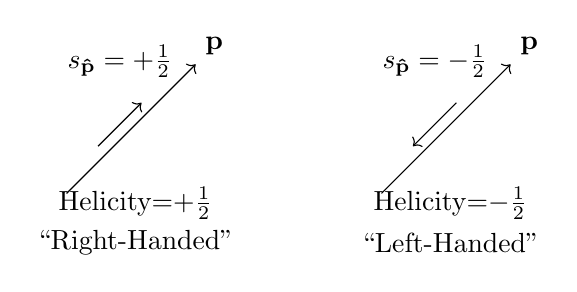
\begin{tikzpicture}[scale=2.0]
    \node (A) at (0,0) {};
    \node (B) at (1,1) {$\vb{p}$};
    \node (Aspin) at (0.4,0.9) {$s_{\vu{p}}=+\frac12$};
    \node (Ap) at (0.2,0.3) {};
    \node (Bp) at (0.6,0.7) {};
    \node (C) at (2,0) {};
    \node (D) at (3,1) {$\vb{p}$};
    \node (Cspin) at (2.4,0.9) {$s_{\vu{p}}=-\frac12$};
    \node (Cp) at (2.2,0.3) {};
    \node (Dp) at (2.6,0.7) {};
    \draw [->] (A) -- (B);
    \draw [->] (Ap) -- (Bp);
    \draw [->] (C) -- (D);
    \draw [<-] (Cp) -- (Dp);
    \node (plus) at (0.5,0) {Helicity=$+\frac12$};
    \node (minus) at (2.5,0) {Helicity=$-\frac12$};
    \node (plusT) at (0.5,-0.25) {``Right-Handed''};
    \node (minusT) at (2.5,-0.25) {``Left-Handed''};
  \end{tikzpicture}
  \caption{Helicity demo}
  \label{fig:helicity}
\end{figure}
The helicity of a \underline{massless} particle is a Lorentz invariant, i.e. the same in all frames: helicity $= \frac12\bm\sigma\vdot\vu{p}$.

Look closer at QCD: It conserves helicity:
\begin{figure}[H]
  \centering
  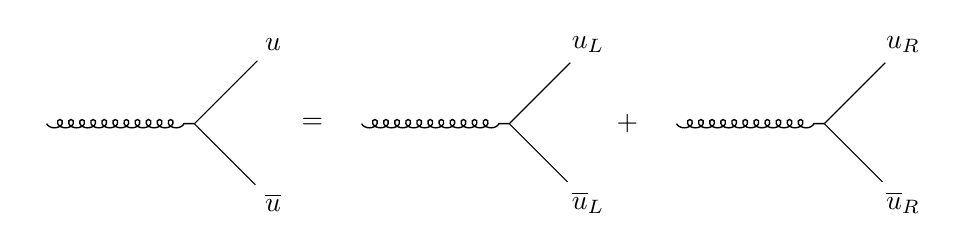
\begin{tikzpicture}[scale=2.0]
    \begin{feynhand}
      % Symbols
      \vertex (eq) at (1.75,0) {=};
      \vertex (pl) at (3.75,0) {+};
      % vertices
      \vertex (p11) at (1.5,0.5) {$u$};
      \vertex (p12) at (1.5,-0.5) {$\bar{u}$};
      \vertex (a1) at (0,0) {};
      \vertex (b1) at (1,0);
      % propagators
      \propag [gluon] (a1) to (b1);
      \propag (b1) to (p11);
      \propag (b1) to (p12);
      % vertices
      \vertex (p21) at (3.5,0.5) {$u_L$};
      \vertex (p22) at (3.5,-0.5) {$\bar{u}_L$};
      \vertex (a2) at (2,0) {};
      \vertex (b2) at (3,0);
      % propagators
      \propag [gluon] (a2) to (b2);
      \propag (b2) to (p21);
      \propag (b2) to (p22);
      % vertices
      \vertex (p31) at (5.5,0.5) {$u_R$};
      \vertex (p32) at (5.5,-0.5) {$\bar{u}_R$};
      \vertex (a3) at (4,0) {};
      \vertex (b3) at (5,0);
      % propagators
      \propag [gluon] (a3) to (b3);
      \propag (b3) to (p31);
      \propag (b3) to (p32);
    \end{feynhand}
  \end{tikzpicture}
  \caption{QCD Conservation of Helicity}
  \label{fig:qcdhelicity}
\end{figure}
Due to the time conventions, this interation looks like:
\begin{figure}[H]
  \centering
  \begin{tikzpicture}[scale=2.0]
    \begin{feynhand}
      % vertices
      \vertex (u1) at (0,0) {$u_L$};
      \vertex (u2) at (2,0) {$u_L$};
      \vertex (a) at (1,0);
      \vertex (b) at (1,-1);
      % propagators
      \propag [gluon] (a) to (b);
      \propag [mom'={}] (a) to (u1);
      \propag [mom'={}] (u2) to (a);
    \end{feynhand}
  \end{tikzpicture}
  \caption{Equivalent to \ref{fig:qcdhelicity}}
  \label{fig:qcdhelicity2}
\end{figure}
Replacing the $u$ with $d$ gives the same $SU(2)$ structure, except for each of the left and right helicity particles, giving an $SU(2)_L$ and $SU(2)_R$. So the full symmetry of QCD is:
\begin{align*}
  SU(2)_{L}\otimes SU(2)_{R}
\end{align*}
Which better represents the chiral symmetry.

We saw that $SU(2)_{isospin}$ led to three pions of equal mass, ($\pi^+,\pi^0,\pi^-$). But the symmetry of QCD is bigger than $SU(2)_I$; why is it not manifest in the particle spectrum? Because $SU(2)_L\otimes SU(2)_R$ is spontaneously broken! This means we really see $SU(2)_I$ as a ``hidden'' version of $SU(2)_L\otimes SU(2)_R$, that is $SU(2)_L\otimes SU(2)_R\to SU(2)_I$. Since we lose 3 degrees of freedom from this ($SU(2)_L\otimes SU(2)_R$ has 6, $SU(2)_I$ has 3).

Recall scalar field: $\phi\to e^{i\alpha}\phi$ under $U(1)$. Since the symmetry is broken or hidden, the ground state value should not obey this $U(1)$, i.e. it is not at $\phi=0$, so assume:
\begin{align*}
  \ev{\phi}_0&=\frac{v}{\sqrt{2}}\\
  \implies\ev{\phi}_0\to e^{i\alpha}\ev{\phi}_0
\end{align*}
This creates a Goldstone Boson!

For quarks, the chirality means they act as a doublet:
\begin{align*}
  q\equiv\pmqty{u\\d}
\end{align*}
And each left/right doublet acts differently under its own $SU(2)_{L/R}$:
\begin{align*}
  SU(2)_L&: q_L\to U_Lq_L, \bar{q}_L\to\bar{q}_LU_L^\dag\\
  U_L&=e^{i\sigma\alpha_L}\in SU(2)_L\\
  SU(2)_R&: q_R\to U_Rq_R, \bar{q}_R\to\bar{q}_RU_R^\dag\\
  U_R&=e^{i\sigma\alpha_R}\in SU(2)_R
\end{align*}

The QCD force produces a condensate:
\begin{align*}
  \ev{\bar{q}q}_0\neq0\implies \ev{\bar{q}_Lq_R+\bar{q}_Rq_L}\neq 0
\end{align*}
This fact breaks BOTH $SU(2)_L$ and $SU(2)_R$:
\begin{align*}
  \ev{\bar{q}_Lq_R+\bar{q}_Rq_L}\underset{SU(2)_L}{\to}
  \bar{q}_LU^\dag_Lq_R+\bar{q}_RU_Lq_L\\
  \ev{\bar{q}_Lq_R+\bar{q}_Rq_L}\underset{SU(2)_R}{\to}
  \bar{q}_LU_Rq_R+\bar{q}_RU^\dag_Rq_L
\end{align*}
So it appears we have kept neither $SU(2)_L$ nor $SU(2)_R$ on their own. Consider rotation by \underline{both} $U_L$ and $U_R$ at the same time and by the same amount, this means $U_L=U_R$, so we get:
\begin{align*}
  \ev{\bar{q}_Lq_R+\bar{q}_Rq_L}\underset{SU(2)_L\otimes SU(2)_R}{\to}
  \bar{q}_L\underbrace{U^\dag_LU_R}_{\bm{1}}q_R+
  \bar{q}_R\underbrace{U^\dag_RU_L}_{\bm{1}}q_L
  =\ev{\bar{q}_Lq_R+\bar{q}_Rq_L}
\end{align*}
Hence, there is an unbroken combination of $SU(2)_L\otimes SU(2)_R$ with $U=U_L=U_R$ that leaves an $SU(2)$ we call isospin! Chiral symmetry breaking is then represented by $SU(2)_L\otimes SU(2)_R\to SU(2)_I$. There are 3 broken symmetries, which lead to our 3 Goldstone bosons $(\pi^+,\pi^0,\pi^-)$. The 3 unbroken symmetries give the remaining Isospin symmetry.


\subsection{Pion Field Theory}
Effective theory of $SU(2)_L\otimes SU(2)_R\to SU(2)_I$:

This is a model of spin-0 fields which displays chiral symmetry breaking -- also called a \underline{``$\sigma$ model''}.

Consider $\phi=\pmqty{a\\b}$, with $a,b\in\mathbb{C}$, so a complex doublet with \underline{4 degrees of freedom}. The Lagrangian is given by:
\begin{align*}
  \L=\D_\mu\phi^\dag\D^\mu\phi-V(\phi^\dag\phi)
\end{align*}
The Lagrangian is invariant under $\phi\to U\phi$ with $U\in SU(2)$.
In fact, the symmetry is even larger. To see this, think of $\phi$ as a matrix:
\begin{align*}
  \Phi &= \pmqty{a&-b^*\\b&a^*}\\
  \phi^\dag\phi&=\abs{a}^2+\abs{b}^2\\
  \Phi^\dag\Phi&=\pmqty{\abs{a}^2+\abs{b}^2\\&\abs{a}^2+\abs{b}^2}\\
  \implies\frac12\Tr[\Phi^\dag\Phi]&=\abs{a}^2+\abs{b}^2
\end{align*}
So rewrite the Lagrangian in terms of $\Phi$:
\begin{align*}
  \L=\frac12\Tr[\D_\mu\Phi^\dag\D^\mu\Phi]-V\qty(\frac12\Tr[\Phi^\dag\Phi])
\end{align*}
Note that $\det\Phi$ also is $\abs{a}^2+\abs{b}^2$, so we have the constraint that:
\begin{align*}
  \det\Phi=\frac12\Tr[\Phi^\dag\Phi]
\end{align*}
This Lagrangian obeys 2 very different symmetries:
\begin{align*}
  \Phi\to U_L\Phi\quad U_L\in SU(2)_L\\
  \Phi\to \Phi U_R^\dag\quad U_R\in SU(2)_R
\end{align*}

Lets get to the symmetry breaking. Let $\ev{\Phi}_0\neq0$, specifically choose $a=\frac{v}{\sqrt{2}},b=0$, or:
\begin{align*}
  \ev{\Phi}_0=\frac1{\sqrt{2}}\pmqty{v\\&v}
\end{align*}
This is the same story and physics as before, transform this under the combination $SU(2)_L\otimes SU(2)_R$
\begin{align*}
  \ev{\Phi}_0\underset{SU(2)_L\otimes SU(2)_R}{\to}
  U_L\ev{\Phi}_0U^\dag_R=\frac1{\sqrt{2}}\pmqty{v\\&v}U_LU_R^\dag
\end{align*}
We can exchange $\ev{\phi_0}$ and $U_L$ since it is proportional to the identity. This will only go back to $\ev{\Phi}_0$ if $U_L=U_R$, the rotations are by the same amount. This is the isospin again!

As before, consider the shifted field with a zero vacuum expectation value (vev):
\begin{align*}
  \Phi=\frac1{\sqrt{2}}\pmqty{\sigma+v\\&\sigma+v}
  \exp[\frac{i}2\bm{\tau}\vdot\bm{\pi}]
\end{align*}
Where $\tau_i$ are the Pauli Matrices, and $\pi_i$ are the pion fields. Note that $\sigma$ are \emph{not} the pauli matrices, they are another field. This time the potential becomes:
\begin{align*}
  V&=\lambda\qty(\frac12\Tr\Phi^\dag\Phi-\frac{v^2}2)^2\\
  &=\lambda\qty(\frac122\frac12(\sigma+v)^2-\frac{v^2}2)^2\\
  &=\lambda\qty(\frac12\sigma^2+\sigma v)^2
\end{align*}
Notice that the pion fields disappear from the trace due to them being completely in the exponential. This means that $\pi_i$ are massless Goldstone bosons, with ($i=1,2,3$).

Under Isospin, we have:
\begin{align*}
  \Phi&=\frac1{\sqrt{2}}\pmqty{\sigma+v\\&\sigma+v}e^{i/2 \tau\vdot\pi}\\
  U\Phi U^\dag=\frac1{\sqrt{2}}\pmqty{\sigma+v\\&\sigma+v}
  Ue^{i/2\tau\vdot\pi}U^\dag
\end{align*}
The remaining part, $Ue^{i/2\tau\vdot\pi}U^\dag$, can be written as $e^{i/2\tau\vdot\pi'}$, where $\pi_i'$ are rotated $\pi$ fields.

The Physics of the $\sigma$ field is a bit murky. We see it in a broad enhancement in $\pi\pi$ scattering, so we see something like $\pi\pi\to\sigma\to\pi\pi$.

But the $\sigma$ is not in the Particle Data Book, but that just means its existence is not unambiguous. What even is a particle?

\subsection{Strangeness and $SU(3)$}
Lets add the strange quark to the discussion:
\begin{align*}
  \pmqty{u\sim\SI{4}{\MeV}\\d\sim\SI{7}{\MeV}\\s\sim\SI{150}{\MeV}\\}
\end{align*}
The charge of $s$ is $-\frac{1}{3}$, so it is not a triplet of EM, but rather it is a triplet of a new flavor, $SU(3)$. Note that we were able to ignore this quark model and work with the broken chiral symmetry of $SU(2)_I$ since the mass of the $u$ and $d$ were much less than the mass of the constituent particles we were dealing with. So approximating the full QCD as just $SU(3)$ will not be as good of an approximation since $m_s$ is so large. 

Recall that the pions all had $I=1$ and corresponded to the triplet states of adding two $I=1/2$ particles, the missing $I=0$ state involves the strange quark and is the $\eta(547)=\frac1{\sqrt{6}}\qty(u\bar{u}-d(-\bar{d})-2s\bar{s})$. Thus means that the $s$ quark is an isospin singlet.

\subsubsection{New Mesons}
We have a couple new mesons corresponding to our new quark:
\begin{itemize}
\item The $d$ and $\bar{s}$ make a $K^0$, and its antiparticle $-\bar{d}$ and $s$ make a $\bar{K}^0$, with mass \SI{497.6}{\MeV}
\item The corresponding positively charged particle is from the $u$ and $\bar{s}$, the $K^+$, with mass \SI{493.6}{\MeV}
\item The corresponding negatively charged particle is from the $\bar{u}$ and $s$, the $K^-$, with mass \SI{493.6}{\MeV}
\end{itemize}
$K_0$ and $K^+$ form an isospin doublet, as do $\bar{K}^0$ and $K^-$, but how do they $K$'s fit together with the $\pi$'s under $SU(3)$?

\subsubsection{Fundamental Representation of $SU(3)$}
The fundamental representation of $SU(3)$ is $3\times3$ unitary matrix $U=e^{i\theta\vdot T}$ with $\det{U}=1$, this gives 9-1=8 generators $T$. The parameters $\theta\vdot T=\theta^AT^A$, $A=1,\dots,8$. So $SU(3)$ is 8-dimensional, and the 3-dimensional represetation much satisfy the Lie Algebra $\comm{T^A}{T^B}=if^{ABC}T^C$ relation. One such representation is:
\begin{align*}
  T^1&=\frac12\pmqty{0&1&0\\1&0&0\\0&0&0}\quad
  T^2=\frac12\pmqty{0&-i&0\\i&0&0\\0&0&0}\quad
  T^3=\frac12\pmqty{1&0&0\\0&-1&0\\0&0&0}\quad
  T^4=\frac12\pmqty{0&0&1\\0&0&0\\1&0&0}\\
  T^5&=\frac12\pmqty{0&0&-i\\0&0&0\\i&0&0}\quad
  T^6=\frac12\pmqty{0&0&0\\0&0&1\\0&1&0}\quad
  T^7=\frac12\pmqty{0&0&0\\0&0&-i\\0&i&0}\quad
  T^8=\frac1{2\sqrt{3}}\pmqty{1&0&0\\0&1&0\\0&0&-2}
\end{align*}
Notice that the pauli matrices $\sigma$ are embedded inside this larger group. Also notice that $\Tr[T^A]=0$.

This gives us an explicit representation, but the group is identified by the totally antisymmetric structure constants $f^{ABC}$:
\begin{itemize}
\item There are $8\times8\times8=512$ constants here!
\item Of course if $A=B$, $A=C$ or $B=C$, they are 0 by symmetry
\item The non-zero ones are:
  \begin{align*}
    f^{123}&=1\quad(\text{convention})\\
    f^{147}&=f^{246}=f^{257}f^{345}=f^{516}=f^{637}=\frac12\\
    f^{458}&=f^{678}=\frac{\sqrt{3}}{2}
  \end{align*}
  You can get the rest through the antisymmetric property
\end{itemize}
So, the quark triplet $\pmqty{u&d&s}$ is transformed under the fundamental representation given by the $T^A$ above. The antiquark triplet $\pmqty{\bar{u}&\bar{d}&\bar{s}}$ transforms under the complex conjugate representation, $-(T^A)^*$. However unlike $SU(2)$, this representation is not unitarily equivalent to the fundamental representation.
The fundamenetal representation is called a $3$, and its unrelated complex conjugate is a $\bar{3}$
While the quarks and antiquarks transform under 3 and $\bar{3}$, respectively, the $\pi$'s and $K$'s transform under a different representation called the \emph{adjoint} representation.
The adjoint representation must satify the Lie Algebra $\comm{T^A}{T^B}=if^{ABC}T^C$. Think of $(f^A)^{BC}$ as a set of $A=1,\dots,N$ matrices of dimension $N\times N$, (For $SU(3)$, $N=8$). A convenient way to construct the adjoint generators is to choose $(T^A)^{BC}=-if^{ABC}$.

\begin{definition}[Adjoint Representation]
  The dimension of an adjoint representation has the same dimension as the group
\end{definition}
Lets plug in to $\comm{T^A}{T^B}=if^{ABC}T^C$:
\begin{align*}
  (T^A)^{DE}(T^B)^{EF}-(T^B)^{DE}(T^A)^{EF}&=if^{ABC}(T^C)^{DF}\\
  \implies -f^{ADE}f^{BEF}+f^{BDE}f^{AEF}&=f^{ABC}f^{CDF}\\
  \implies f^{ADE}f^{EBF}+f^{BDE}f^{AEF}&+f^{BAE}f^{EDF}=0
\end{align*}
This important relation is called the Jacobi identity. So we have shown these matrices $(T^A)^{BC}$ satisfy the Lie Algebra, and form the adjoint representation.

The $\pi$'s and $K$'s transform as an octet (8) under this representation. This is usually displayed as:
\begin{figure}[H]
  \centering
  \begin{tikzpicture}
    % axes
    \draw[latex-latex, thin, draw=gray] (-2.4,0)--(2.4,0) node [right] {$I$};
    \draw[latex-latex, thin, draw=gray] (0,-2.4)--(0,2.4) node [above] {$s$};
    % positions on axes
    \node at (-0.75, 1.3) {\textbullet};
    \node at (-0.75, 1.3) [above] {\(K^0\)};
    \node at ( 0.75, 1.3) {\textbullet};
    \node at ( 0.75, 1.3) [above] {\(K^+\)};
    \node at (-0.75,-1.3) {\textbullet};
    \node at (-0.75,-1.3) [below] {\(K^-\)};
    \node at ( 0.75,-1.3) {\textbullet};
    \node at ( 1.0,-1.3) [below] {\(\overline{K}^0\)};
    \node at (-1.5, 0.0) {\textbullet};
    \node at (-1.5, 0.0) [below] {$\pi^-$};
    \node at ( 0.0, 0.0) {\textbullet};
    \node at ( 0.0, 0.0) [below] {$\pi^0$};
    \node at ( 1.5, 0.0) {\textbullet};
    \node at ( 1.5, 0.0) [below] {$\pi^+$};
    \node at ( 0.1, 0.1) {\textbullet};
    \node at ( 0.1, 0.1) [above] {$\eta(547)$};
    % strangeness labels
    \node at (-2.9, 0.0) {$s=0$};
    \node at (-2.9, 1.3) {$s=+1$};
    \node at (-2.9,-1.3) {$s=-1$};
  \end{tikzpicture}
  \caption{Strangeness and Isospin Plot}
  \label{fig:strangeisospin}
\end{figure}
We fill out the octet with the $I=0$ meson $\eta(547)$. The $\eta$ mass is dominated by the strange quarks inside.

Note: It is a historical accident that the $s$ quark has $S=-1$, and $\bar{s}$ has $S=1$.

The quark content of each of these is:
\begin{gather*}
  K^+=u\bar{s}\qquad \bar{K}^0=-\bar{d}s\quad K^0=d\bar{s}\quad K^-=\bar{u}s\\
  \eta=\frac1{\sqrt{6}}(u\bar{u}+d\bar{d}-2s\bar{s})
\end{gather*}
Notice the structure of $\eta$'s quark content is similar to the generator $T^8$, similarly, $\pi^0$ is similar to $T^3$ in the fundamental representation. Mesons are $q\bar{q}$, so we have $3\otimes\bar{3}=8\oplus1$. Where the $3$ represents a quark, $\bar{3}$ an antiquark.

Just like $SU(2)_L\otimes SU(2)_R\to SU(2)_I$, we now have a larger $SU(3)_L\otimes SU(3)_R$ being broken, this time to $SU(3)$ and 8 broken generators, where $\pi$, $\kappa$, and $\eta$ are the pseudo-goldstone bosons.
The singlet state is $\eta'(958)=\frac1{\sqrt{3}}(u\bar{u}+d\bar{d}+s\bar{s})$, Why is the mass so large? $\eta'(958)$ is a goldstone boson of $U(1)_{Axial}$, should be ~massless:
\begin{align*}
  q_L\to e^{i\alpha_L}q_L,\quad q_R\to e^{i\alpha_R}q_R\\
  \alpha_L=\alpha_R\implies \text{Baryon Number}\\
  \alpha_L=-\alpha_R\implies \text{Axial $U(1)$}
\end{align*}
This $U(1)_A$ is broken by the vacuum meson state $\ev{\bar{q}q}_0$.

$U(1)_A$ is \emph{not} a symmetry due to a quantum field theoretic anomaly (quantum effects do not preserve the symmetry). This implies $\eta'$ is \emph{not} a goldstone boson. Its mass comes from a topological effect of field configurations called instantons.

\subsubsection{$J=1$ Mesons}

\begin{figure}[H]
  \centering
  \begin{tikzpicture}
    % positions on axes
    \node at (-0.75, 1.3) {\textbullet};
    \node at (-0.75, 1.3) [above] {\(K^{*0}\)};
    \node at ( 0.75, 1.3) {\textbullet};
    \node at ( 0.75, 1.3) [above] {\(K^{*+}\)};
    \node at (-0.75,-1.3) {\textbullet};
    \node at (-0.75,-1.3) [below] {\(K^{*-}\)};
    \node at ( 0.75,-1.3) {\textbullet};
    \node at ( 1.0,-1.3) [below] {\(\overline{K}^{*0}\)};
    \node at (-1.5, 0.0) {\textbullet};
    \node at (-1.5, 0.0) [below] {$\rho^-$};
    \node at ( 0.0, 0.0) {\textbullet};
    \node at ( 0.0, 0.0) [below] {$\rho^0$};
    \node at ( 1.5, 0.0) {\textbullet};
    \node at ( 1.5, 0.0) [below] {$\rho^+$};
    \node at ( 0.1, 0.1) {\textbullet};
    \node at ( 0.1, 0.1) [above] {$\omega_8$};
    % strangeness labels
    \node at (-2.9, 0.0) {$s=0$};
    \node at (-2.9, 1.3) {$s=+1$};
    \node at (-2.9,-1.3) {$s=-1$};
  \end{tikzpicture}
  \caption{Strangeness/Isospin Octet with $J=1$}
  \label{fig:strangeisospin2}
\end{figure}
Note the mass of $K^*(894)$ and $\rho(775)$.

Similar to the $\eta$ with $J=0$, the $J=1$ $\omega_8=\frac1{\sqrt{6}}(u\bar{u}+d\bar{d}-2s\bar{s})$. Much like the $\eta'$, the singlet is $\omega_1=\frac1{\sqrt{3}}(u\bar{u}+d\bar{d}+s\bar{s})$.

In Nature, $\omega_1$ and $\omega_8$ mix. The observed states are:
\begin{align*}
  \omega&=\frac1{\sqrt{3}}\omega_8+\sqrt{\frac23}\omega_1=
  \frac1{\sqrt{2}}(u\bar{u}+d\bar{d})\\
  \phi&=-\sqrt{\frac23}\omega_8+\frac1{\sqrt{3}}=s\bar{s}
\end{align*}
The mass of $\omega(783)$ and $\phi(1020)$.

Notice in these states, the $(u,d)$ and $s$ separate from each other.


\subsubsection{Strange Baryons}
Recall $SU(2)_I$ Baryons, we had $2\otimes2\otimes2=4\oplus 2_S\oplus 2_A$. The $4$ was the $\Delta$.

Perform the same construction for $SU(3)$. Let 3 representations by $\psi^i$ and $\chi^i$, $i=1,2,3$:
\begin{align*}
  3\otimes3=\psi^i\chi^j=
  \underbrace{\frac12\qty(\psi^i\chi^j+\psi^j\chi^i)}_{S^{ij}\text{ Symmetric}}
  +\underbrace{\frac12\qty(\psi^i\chi^j-\psi^j\chi^i)}_{A^{ij}\text{ Antisymmetric}}
\end{align*}
Note that $S^{ij}$ is a $3\times3$ symmetric matrix with 6 independent elements, and $A^{ij}$ is a $3\times3$ antisymmetric matrix with 3 independent elements. This means $3\otimes3=6\oplus\bar{3}$, the $\bar{3}$ is not obvious here.

Add one quark:
\begin{align*}
  3\otimes(3\otimes3)=3\otimes(6\oplus\bar{3})
\end{align*}
Break this into pieces:
\begin{enumerate}
\item $3\otimes6$:
  \begin{align*}
    \psi^kS^{ij}&=\frac12\qty(\psi^kS^{ij}+\psi^iS^{kj}+\psi^jS^{ik})
    +\frac12\qty(\psi^kS^{ij}-\psi^iS^{kj}-\psi^jS^{ik})\\
    &=S^{kij}+M^{kij}
  \end{align*}
  Where $S^{ijk}$ is a totally symmetric matrix, with 10 independent elements, and $M^{kij}$ is symmetric only on $i\iff j$, so $8$ independent elements.

  The end result is $3\otimes 6=10\oplus 8$
\item $3\otimes\bar{3}=8\oplus 1$ we know from mesons
\end{enumerate}
Thus we get $3\otimes 3\otimes 3=10_s\oplus8_M\oplus8_M\oplus1$, a decuplet, 2 octets, and a singlet.
\begin{figure}[H]
  \centering
  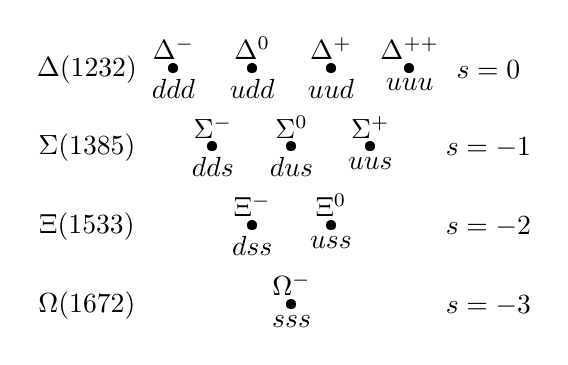
\begin{tikzpicture}
    % labels for each particle
    \node at ( 0.0, 3.0) {$\Delta(1232)$};
    \node at ( 0.0, 2.0) {$\Sigma(1385)$};
    \node at ( 0.0, 1.0) {$\Xi(1533)$};
    \node at ( 0.0, 0.0) {$\Omega(1672)$};
    % s=0 Deltas
    \node at ( 1.1, 3.0) {\textbullet};
    \node at ( 1.1, 3.0) [above] {$\Delta^-$};
    \node at ( 1.1, 3.0) [below] {$ddd$};
    \node at ( 2.1, 3.0) {\textbullet};
    \node at ( 2.1, 3.0) [above] {$\Delta^0$};
    \node at ( 2.1, 3.0) [below] {$udd$};
    \node at ( 3.1, 3.0) {\textbullet};
    \node at ( 3.1, 3.0) [above] {$\Delta^+$};
    \node at ( 3.1, 3.0) [below] {$uud$};
    \node at ( 4.1, 3.0) {\textbullet};
    \node at ( 4.1, 3.0) [above] {$\Delta^{++}$};
    \node at ( 4.1, 3.0) [below] {$uuu$};
    % s=-1 sigma
    \node at ( 1.6, 2.0) {\textbullet};
    \node at ( 1.6, 2.0) [above] {$\Sigma^-$};
    \node at ( 1.6, 2.0) [below] {$dds$};
    \node at ( 2.6, 2.0) {\textbullet};
    \node at ( 2.6, 2.0) [above] {$\Sigma^0$};
    \node at ( 2.6, 2.0) [below] {$dus$};
    \node at ( 3.6, 2.0) {\textbullet};
    \node at ( 3.6, 2.0) [above] {$\Sigma^+$};
    \node at ( 3.6, 2.0) [below] {$uus$};
    % s=-2 cascade
    \node at ( 2.1, 1.0) {\textbullet};
    \node at ( 2.1, 1.0) [above] {$\Xi^-$};
    \node at ( 2.1, 1.0) [below] {$dss$};
    \node at ( 3.1, 1.0) {\textbullet};
    \node at ( 3.1, 1.0) [above] {$\Xi^0$};
    \node at ( 3.1, 1.0) [below] {$uss$};
    % s=-3 omega
    \node at ( 2.6, 0.0) {\textbullet};
    \node at ( 2.6, 0.0) [above] {$\Omega^-$};
    \node at ( 2.6, 0.0) [below] {$sss$};
    % Strangeness labels
    \node at ( 5.1, 3.0) {$s= 0$};
    \node at ( 5.1, 2.0) {$s=-1$};
    \node at ( 5.1, 1.0) {$s=-2$};
    \node at ( 5.1, 0.0) {$s=-3$};
  \end{tikzpicture}
  \caption{Baryon Decuplet $J=\frac32$}
  \label{fig:decuplet}
\end{figure}
Remember, states are symmetrized, e.g.: $\Sigma^0=(dus+dsu+uds+usd+sud+sdu)/\sqrt{6}$.

Also as an aside, the $\Xi$ is not ``xi'' but rather ``cascade''

\begin{figure}[H]
  \centering
  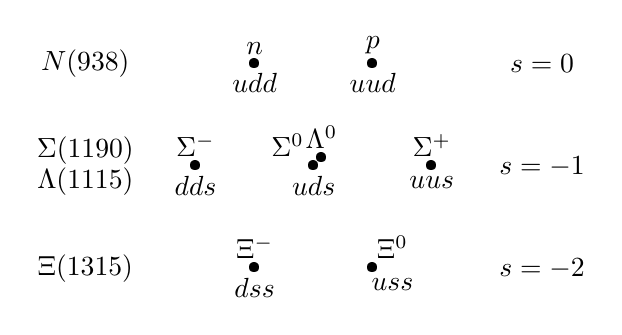
\begin{tikzpicture}
    % positions on axes
    \node at (-0.75, 1.3) {\textbullet};
    \node at (-0.75, 1.3) [above] {$n$};
    \node at (-0.75, 1.3) [below] {$udd$};
    \node at ( 0.75, 1.3) {\textbullet};
    \node at ( 0.75, 1.3) [above] {$p$};
    \node at ( 0.75, 1.3) [below] {$uud$};
    \node at (-0.75,-1.3) {\textbullet};
    \node at (-0.75,-1.3) [above] {$\Xi^-$};
    \node at (-0.75,-1.3) [below] {$dss$};
    \node at ( 0.75,-1.3) {\textbullet};
    \node at ( 1.0,-1.3) [above] {$\Xi^{0}$};
    \node at ( 1.0,-1.3) [below] {$uss$};
    \node at (-1.5, 0.0) {\textbullet};
    \node at (-1.5, 0.0) [above] {$\Sigma^-$};
    \node at (-1.5, 0.0) [below] {$dds$};
    \node at ( 0.0, 0.0) {\textbullet};
    \node at ( 0.0, 0.0) [above left] {$\Sigma^0$};
    \node at ( 0.0, 0.0) [below] {$uds$};
    \node at ( 1.5, 0.0) {\textbullet};
    \node at ( 1.5, 0.0) [above] {$\Sigma^+$};
    \node at ( 1.5, 0.0) [below] {$uus$};
    \node at ( 0.1, 0.1) {\textbullet};
    \node at ( 0.1, 0.1) [above] {$\Lambda^0$};
    % particle labels
    \node at (-2.9, 1.3) {$N(938)$};
    \node at (-2.9, 0.2) {$\Sigma(1190)$};
    \node at (-2.9,-0.2) {$\Lambda(1115)$};
    \node at (-2.9,-1.3) {$\Xi(1315)$};
    % strangeness
    \node at (2.9, 1.3) {$s= 0$};
    \node at (2.9, 0.0) {$s=-1$};
    \node at (2.9,-1.3) {$s=-2$};
  \end{tikzpicture}
  \caption{Baryon Octet $J=\frac12$}
  \label{fig:octet}
\end{figure}
These states must be symmetrized in flavor an spin (like $p,n$). Generally you just replace $u,d$ with $s$. $\Sigma^0$ can be found from $\Sigma^-$ via isospin; $\Lambda^0$ is orthogonal to $\Sigma^0$.

Note: Do not confuse the $J=\frac32$ particles with the $\frac12$ ones, despite their names being similar, they are different.

\subsection{Beyond $SU(3)$}
Adding a charm quark $c$ leads to an $SU(4)$, see Particle Data Group. While the symmetry increases, but now badly broken. If $m_c\sim\SI{1.5}{\GeV}$, this is comparable to hadron masses.

Adding the bottom quark $b$ gives $SU(5)$, $m_b\sim\SI{4.5}{\GeV}$. The $b$ baryons found in 2006, $\Sigma_b(5810), \Sigma_b^*(5830)$, then in 2007, the $\Xi^-_b(5793)$

Adding a top quark does NOT give $SU(6)$, but $m_t\sim\SI{175}{\GeV}$. The top quark decays before it can hadronize.

There are a lot of other possible states -- orbital and/or radial excitations of those we've explored.

There also appear to be ``exotics'': E.g. $f_0(980)$ is believed to be a $K\bar{K}$ bound state (``molecule''), as its mass is very close to $2m_K=\SI{990}{\MeV}$. There was lots of excitement about possible ``pentaquark'' states -- $qqqq\bar{q}$, they seemed too narrow (width) for molecuules, but really were baryons and mesons very close.

There have been many statistically ``significant'' exotics identified over the years ... many have gone away.

\subsection{Beyond Stamp Collectings}

\subsubsection{Masses}
How do we find quark masses?
\begin{enumerate}
\item $\frac{m_\pi^2}{m_K^2}=\frac{ud}{us}$ This gives an estimate for the ratio of the first generation ($u,d$) quarks average mass to the mass of the strange.
\item We can use measurements of the $\Delta^{++}$ and $\Sigma^+$ to get measurements of the strange mass since it would clearly dominated by the strange, so $m_s\sim\SI{150}{\MeV}$
\item We can then get that the average mass of $u,d$ should be $\SI{6}{\MeV}$
\item We can then use the mass measurements of the $K^0$ and $K^+$ to get the ratio of the $u/d$, and find that $m_u\sim\SI{4}{\MeV}$ and $m_d\sim\SI{7}{\MeV}$
\end{enumerate}

We can estimate $m_c$ and $m_b$ best from heavy-quark effective theory (HQET) and now lattice QCD calculations.

$m_t$ can be directly reconstructed from decay products.

\paragraph{Hadron masses} For hadrons with zero orbital angular momenta, the interaction between quarks can depend on the relative orientation of their spins. An empirical expression for meson and baryon masses is:
\begin{align*}
  M_{\text{meson}}&=m_1+m_2+a\frac{\bm{\sigma}_1\vdot\bm{\sigma}_2}{m_1m_2}\\
  M_{\text{baryon}}&=m_1+m_2+m_3+\frac{a'}{2}\sum_{i>j}
  \frac{\bm{\sigma}_i\vdot\bm{\sigma}_j}{m_im_j}
\end{align*}
The dot product $\bm{\sigma}_i\vdot\bm{\sigma}_j$ is the QCD analog of the ``hyperfine'' interaction in QED.

For mesons:
\begin{align*}
  \bm{\sigma}_1\vdot\bm{\sigma}_2&=4(\vb{s}_1\vdot\vb{s}_2)
  =2\qty[(\vb{s}_1+\vb{s}_2)^2-\abs{\vb{s}_1}^2-\abs{\vb{s}_2}^2]\\
  &=2\qty[s(s+1)-s_1(s_1+1)-s_2(s_2+1)]=2\qty[s(s+1)-\frac32]=
  \begin{cases}
    1 & s=1 \\ -3 & s=0
  \end{cases}
\end{align*}
Assuming constituent $m_u=m_d=\SI{310}{\MeV}$, $m_s=\SI{483}{\MeV}$ and $a=\SI{160}{\MeV}$, we get the following calculated masses:
\begin{table}[H]
\centering
\begin{tabular}{c|cccccc}
(\si{\MeV}) & $\pi^\pm$ & $\rho$ & $K$ & $K^*$ & $\eta$ & $\phi$ \\ \hline
Calculated  & 140       & 780    & 484 & 890   & 559    & 1032   \\
Observed    & 140       & 776    & 495 & 892   & 549    & 1020  
\end{tabular}
\caption{Calculated vs. Observed Masses}
\label{tab:obs-vs-calc}
\end{table}

\subsubsection{Magnetic Dipole Moments of Hadrons}
Magnetic dipole moment $\bm{\mu}=\frac{Qe}{2m}g\vb{s}$, $m$ is mass, $\vb{s}$ is spin. From Dirac theory for spin-$\frac12$ particles, $g=2$.

For quarks: $\mu_u=\frac{e\hbar}{3m_uc}$, $\mu_d=-\frac{e\hbar}{6m_dc}$, the magnetic moments for the antiparticles are the negative of these.

For Baryons, $\bm{\mu}_B=\sum_{i}\bm{\mu}_i$.

Recall the structure of the up spin proton:
\begin{align*}
  \ket{p\up}&=\frac1{\sqrt{18}}\qty{
    \qty[2u\up u\up d\dn-u\up u\dn d\up-u\dn u\up d\up]+\dots}\\
  \mu_p&=\frac1{18}\qty{4(\mu_u+\mu_u-\mu_d)
    +(\mu_u-\mu_u-\mu_d)+(\mu_u-\mu_u+\mu_d)}\times 3\\
  &=\frac16\qty[8\mu_u-4\mu_d+2\mu_d]=\frac13[4\mu_u-\mu_d]
\end{align*}
We can similarly find $\mu_n$, or just realize from isospin that $\mu_n=\frac13\qty[4\mu_d-\mu_u]$.

If we assume $m_u=m_d$, the $\mu_d=-\frac12\mu_u$, and we predict that $\mu_n/\mu_p=-2/3$.

Experimentally, we find $\mu_p=2.793\qty(\frac{e\hbar}{2m_pc})$ and $\mu_p=-1.913\qty(\frac{e\hbar}{2m_pc})$, so the ratio is $-0.685$, very close to $-2/3$


% -*- TeX-master: "master.tex" -*-
\section{Dirac Equation}
% -*- TeX-master: "master.tex" -*-
\section{Quantum Electrodynamics}
In deriving the Dirac equation, we formed Lorentz invariants out of Dirac spinors such as $\bar{\psi}\psi$.

Under the Lorentz group, $\bar{\psi}\psi$ is a scalar, $\bar{\psi}\gamma^\mu\psi$ is a 4-vector, so $\bar{\psi}\sla{\D}\psi$ is also a scalar.

We want a Lagrangian $\L$ invariant under the Lorentz group:
\begin{align*}
  \L=i\bar{\psi}\sla{\D}\psi-m\bar{\psi}\psi
\end{align*}
Equation of motion comes from the Principle of Least Action:
\begin{align*}
  \fdv{\L}{\bar{\psi}}=0\implies i\sla{D}\psi-m\psi=0
\end{align*}
Recall that the other term from the Euler-Lagrange is just $0$ since theres no derivatives of $\bar{\psi}$.

In addition to the Lorentz group, $\L$ is also invariant under the following symmetry:
\begin{align*}
  \psi&\to e^{iQ\theta}\psi\\
  \bar{\psi}&\to \bar{\psi}e^{-iQ\theta}
\end{align*}
Where $Q\in\mathbb{R}$, a $U(1)$ symmetry.

This is a \underline{global} symmetry, $\theta$ is the same over all spacetime. The symmetry group is $U(1)$. QED is introduced by demanding the $U(1)$ symmetry be \underline{local}, where $\theta=\theta(x)$ can change smoothly.

Clearly $m\bar{\psi}\psi$ is invariant:
\begin{align*}
  m\bar{\psi}\psi\to m\bar{\psi}e^{-iQ\theta(x)}e^{iQ\theta(x)}\psi
  =m\bar{\psi}\psi
\end{align*}
The other term:
\begin{align*}
  i\bar{\psi}\sla{\D}\psi\to
  \bar{\psi}e^{-iQ\theta(x)}\sla{\D}(e^{iQ\theta(x)}\psi)
  &=\bar{\psi}e^{-iQ\theta(x)}e^{iQ\theta(x)}\sla{\D}\psi
  +iQ\bar{\psi}\gamma^\mu\psi(\D_\mu\theta)\\
  &=i\bar{\psi}\sla{\D}\psi+i\bar{\psi}(iQ\sla{\D}\theta)\psi
\end{align*}
Is not invariant.

This is remedied by introducing a new field $A^\mu$, into the Lagrangian, and demanding $A^\mu$ transform in just the right way to cancel the offending term. Try the following:
\begin{align*}
  \L=i\bar{\psi}(+ieQ\sla{A})\psi
\end{align*}
Where $\sla{A}=A_\mu\gamma^\mu$, the photon field

The second term in the transformation of $i\bar{\psi}\sla{\D}\psi$ is cancelled if:
\begin{align*}
  A^\mu\to A^\mu-\frac1e\D^\mu\theta(x)
\end{align*}
This local transformation is called a \underline{gauge} transformation, and we say $\L$ is gauge invariant.

The field $A^\mu$ corresponds to the vector potential of the electromagnetic field, and $eQ$ is the electric charge of the fermion.
\begin{itemize}
\item $e$ is called the coupling constant $\alpha=e^2/4\pi\approx 1/137$ is the fine structure constant
\item $Q$ is the charge of particle in units of $e$, $Q=-1$ for electrons, and $Q=+\frac23$ for up quark, etc.
\end{itemize}
The quantum of the EM field is the photon. A mass term in $\L$ would be:
\begin{align*}
  -\frac12M^2A^\mu A_\mu
\end{align*}
But this is \underline{not} gauge invariant. We regard the masslessness of the photon as being a consequence of gauge invariance (although the inverse transformation is also reasonable).

The photon is a massless spin-1 particle and transforms as the $(1,0)\oplus(0,1)$ representation of the Lorentz group. It therefore as helicity $h=\pm1$.

Due to gauge invariance, $A_\mu\to A_\mu-\frac1e\D_\mu\theta$, we can always find a gauge (some $\theta(x)$) where:
\begin{align*}
  \D_\mu A^\mu=0
\end{align*}
This is called the Lorentz gauge, so called because of its manifest Lorentz invariance.

The photon field is:
\begin{align*}
  A^\mu(x)=\int\frac{\dd[3]{p}}{2E}\qty[
  e^{-ip\vdot x}a_\lambda\veps^\mu_\lambda(p)+
  e^{+ip\vdot x}a^\dag_\lambda\veps^{\mu*}_\lambda(p)
  ]
\end{align*}
Where $a,a^\dag$ are the destruction and creation operators for the photon, and $\veps^\mu_\lambda(p)$ is a four-vector which transforms as either the $(1,0)$ rep ($\lambda=+1$), or the $(0,1)$ rep ($\lambda=-1$) of the Lorentz group.

Recall $\psi(x)$:
\begin{align*}
  \psi(x)=\int\frac{\dd[3]{p}}{2E}\qty[
  e^{-ip\vdot x}a_\lambda u_\lambda(p)+
  e^{+ip\vdot x}b^\dag_\lambda v_\lambda(p)
  ]
\end{align*}
The Lorentz gauge condition implies:
\begin{align*}
  p_\mu\veps^\mu_\lambda(p)=0
\end{align*}
This means $\veps^\mu_\lambda$ is the Fourier transform of the photon field, and implies the photon is its own antiparticle.

The ``polarization vectors'' $\veps^\mu_\lambda$ for a photon with momentum $p^\mu=(E,0,0,E)$ are:
\begin{align*}
  \veps^\mu_+&=\frac1{\sqrt{2}}(0,1,i,0)\\
  \veps^\mu_-&=\frac1{\sqrt{2}}(0,1,-i,0)
\end{align*}

\begin{aside}
  Lorentz group (photon not massless) $\lambda=0,\pm1$, for a real photon we would have to remove $\lambda=0$. The radiation gauge, $A^0=0, \grad_i\vdot A^i$, $\lambda=\pm1$ manifestly.
\end{aside}

\subsection{Perturbation Theory}
QED is a weakly-coupled theory -- photons and electrons (or quarks) do not interact very strongly. To zeroth order they do not interact at all. Hence, one can regard interactions as perturbations of this simple picture. The outcome of treating QED perturbatively can be represented pictorially via Feynman diagrams. These ``Feynman rules'' are derived from quantum field theory. In practice, all one needs for simple calculations are the Feynman rules.

Lets draw the Feynman diagram for $e^+e^-\to\mu^+\mu^-$ then work out the details:
\begin{figure}[H]
  \centering
  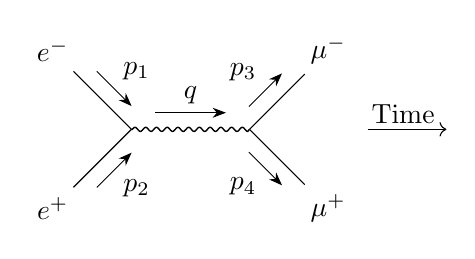
\begin{tikzpicture}
    \begin{feynhand}
      \vertex (a) at (0,0);
      \vertex (e1) at (-1, 1) {$e^-$};
      \vertex (e2) at (-1,-1) {$e^+$};
      \vertex (m1) at (2.5, 1) {$\mu^-$};
      \vertex (m2) at (2.5,-1) {$\mu^+$};
      \vertex (b) at (1.5,0);
      \propag[mom=\(p_1\)] (e1) to (a);
      \propag[mom'=\(p_2\)] (e2) to (a);
      \propag[mom=\(p_3\)] (b) to (m1);
      \propag[mom'=\(p_4\)] (b) to (m2);
      \propag[bos, mom=\(q\)] (a) to (b);
    \end{feynhand}
    \draw[->] (3.0, 0.0) -- (4.0, 0.0);
    \node at (3.45, 0.2) {Time};
  \end{tikzpicture}
  \caption{Feynman Diagram for $e^+e^-\to\mu^+\mu^-$}
\end{figure}

\begin{aside}
  Many older books draw time going up. More modern notation has time flowing to the right. 
\end{aside}

The interaction ``vertex'' (seen below) comes from the Lagrangian:
\begin{align*}
  \L=i\bar{\psi}(\sla{\D}+ieQ\sla{A})\psi-m\bar{\psi}\psi
\end{align*}
\begin{figure}[H]
  \centering
  \begin{tikzpicture}
    \begin{feynhand}
      \vertex (a) at (0,0);
      \vertex (e1) at (-1, 1) {$e^-$};
      \vertex (e2) at (-1,-1) {$e^+$};
      \vertex (b) at (1.5,0) {$\gamma$}; 
      \propag (e1) to (a);
      \propag (e2) to (a);
      \propag[bos] (a) to (b);
    \end{feynhand}
  \end{tikzpicture}
  \caption{The interaction vertex}
\end{figure}
What does this mean?
\begin{itemize}
\item $\psi$ Destorys an $e^-$
\item $\bar{\psi}$ Destorys an $e^+$
\item $A^\mu$ creates a photon ($\gamma$)
\end{itemize}

We can ``read-off'' the Feynman rule for the interaction vertex: (Note that overall sign is convention, not all vertices are simple):
\begin{align*}
  \begin{tikzpicture}[baseline=-0.15cm]
    \begin{feynhand}
      \vertex (a) at (0,0);
      \vertex (e1) at (-1, 1) {$e^-$};
      \vertex (e2) at (-1,-1) {$e^+$};
      \vertex (b) at (1.5,0) {$\gamma$}; 
      \propag[fer] (e1) to (a);
      \propag[antfer] (e2) to (a);
      \propag[bos] (a) to (b);
    \end{feynhand}
  \end{tikzpicture}
  =-ieQ\gamma^\mu
\end{align*}
Where $Q=$ particle charge ($-1$ for $e^-$ and $e^+$).

The second ingredient we need is the ``propagator'' of the photon which mediates the interaction. This is not a real photon. A real photon is not kinematically allowed.
\begin{proof}
  Let the electron and positron 4-momenta respectively be:
  \begin{align*}
    p_1=(E,0,0,p)\qquad p_2=(E,0,0,-p)
  \end{align*}
  And that they are colliding head-on (in c.o.m.\ frame) in an experiment (BEPC, Tristan, CESR, SLAC, LEP, etc.)
  The photon momentum is the sum of these two:
  \begin{align*}
    q_{\gamma}&=p_1+p_2=(2E,0,0,0)\\
    \implies q_{\gamma}^2=4E^2\neq 0
  \end{align*}
  A real photon would have $q^2=0$ always. 
\end{proof}

The interaction is mediated by a ``virtual'' photon (a particle \underline{not} ``on the mass shell'', i.e.\ $q^2\neq m^2$). These ``particles'' do not actually exist in the same sense that real photons (w/ $q^2=0$) do. Also $q^2$ is \underline{not} constrained to be greater than $0$ in general (though it is here).

What is the time scale of this interaction? Dimensional analysis says:
\begin{align*}
  t\sim\frac1{\sqrt{q^2}}\sim\frac1{2E}
\end{align*}
The minimum (threshold) energy for this interaction is that $2E\sim\SI{200}{\MeV}$ Hence $t$ is about:
\begin{align*}
  t\sim\frac{\hbar c}{2Ec}\sim 10^{-23}\text{s}
\end{align*}

When a virtual particle appears in a Feynman diagram, this corresponds to a propagator:
\begin{align*}
  \text{spin 0}\quad
  \begin{tikzpicture}[baseline=-0.10cm]
    \begin{feynhand}
      \vertex (a) at (0,0);
      \vertex (b) at (1.5,0); 
      \propag[sca, mom=\(p\)] (a) to (b);
    \end{feynhand}
  \end{tikzpicture}
  &=\frac{i}{p^2-m^2}\\
  \text{spin }\frac12\quad
  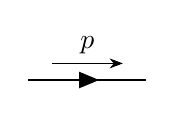
\begin{tikzpicture}[baseline=-0.10cm]
    \begin{feynhand}
      \vertex (a) at (0,0);
      \vertex (b) at (1.5,0); 
      \propag[fer, mom=\(p\)] (a) to (b);
    \end{feynhand}
  \end{tikzpicture}
  &=\frac{i}{\sla{p}-m}=\frac{i(\sla{p}+m)}{p^2-m^2}\\
  \text{(massless) spin 1}\quad
  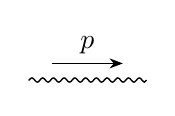
\begin{tikzpicture}[baseline=-0.10cm]
    \begin{feynhand}
      \vertex (a) at (0,0);
      \vertex (b) at (1.5,0); 
      \propag[bos, mom=\(p\)] (a) to (b);
    \end{feynhand}
  \end{tikzpicture}
  &=\frac{i(-g^{\mu\nu}+p^\mu p^\nu/p^2)}{p^2}
\end{align*}
\begin{remark}
  The charge arrow on the fermion above is defined such that the direction of motion of the \emph{particle} is the direction of the charge arrow. \emph{Antiparticles} go backward in time.
\end{remark}

The numerators of the propagators come from summing over helicities:
\begin{align*}
  \sum_{\lambda=\pm}u_\lambda\bar{u}_\lambda&=\sla{p}+m\\
  \sum_{\lambda=\pm,0}\veps^\mu_\lambda\bar{\veps}^\nu_\lambda&=
  -g^{\mu\nu}+\frac{p^\mu p^\nu}{p^2}
\end{align*}

The photon propagator looks complicated, but we will see that the second term will not contribute in practice in either of QED or QCD.

Lets now turn the pictogram into an actual calculation of the scattering amplitude:
\begin{figure}[H]
  \centering
  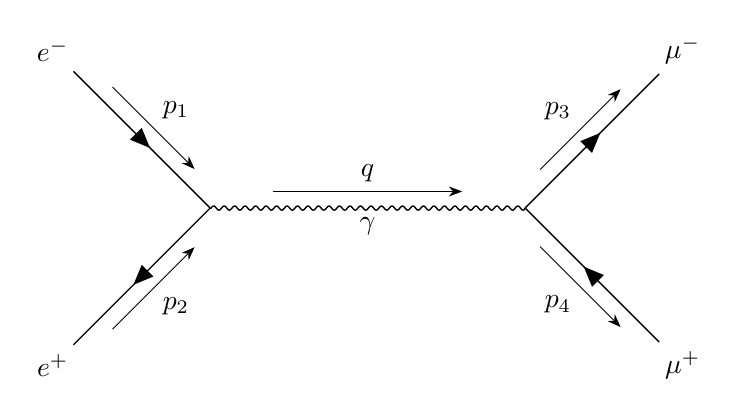
\begin{tikzpicture}[scale=2.0]
    \begin{feynhand}
      % vertices
    \vertex (p11) at (-1,1) {$e^-$};
    \vertex (p12) at (-1,-1) {$e^+$};
    \vertex (p21) at (3,1) {$\mu^-$};
    \vertex (p22) at (3,-1) {$\mu^+$};
    \vertex (a) at (0,0);
    \vertex (b) at (2,0);
    % particles
    \propag [fer, mom=\(p_1\)] (p11) to (a);
    \propag [antfer, mom'=\(p_2\)] (p12) to (a);
    \propag [fer, mom=\(p_3\)] (b) to (p21);
    \propag [antfer, mom'=\(p_4\)] (b) to (p22);
    % propagator
    \propag [bos, mom=\(q\)] (a) to [edge label'=\(\gamma\)] (b);
    \end{feynhand}
  \end{tikzpicture}
  \caption{$e^+e^-\to\mu^+\mu^-$}
  \label{fig:feynman}
\end{figure}
The arrows on the actual edges indicate charge or ``fermion'' flow, read the spinor chain opposite in the direction of these arrows, for example, the left chain would be read as:
\begin{align*}
  \bar{v}(p_2)(-ieQ_e\gamma^\mu)u(p_1)
\end{align*}
And the right chain would read as:
\begin{align*}
  \bar{u}(p_3)(-ieQ_\mu\gamma^\nu)v(p_4)
\end{align*}
The last thing to get is the propagator, then we can write out $\M$, the matrix element:
\begin{align*}
  i\M=&(-ieQ_e)\bar{v}(p_2)\gamma^\mu u(p_1)\\
  \times&\frac{i}{q^2}\qty(-g_{\mu\nu}+\frac{q_\mu q_\nu}{q^2})\\
  \times&(-ieQ_\mu)\bar{u}(p_3)\gamma^\nu v(p_4)
\end{align*}
$\M$ is the amplitude, we will square $\M$ to get the probability that feeds into the cross section or particle decay width.

Lets first show that the second term in the photon propagator does not contribute:
\begin{proof}
  Consider what is actually being calculated:
  \begin{align*}
    \bar{v}(p_2)\gamma^\mu u(p_1)q_\mu=\bar{v}(p_2)\sla{q}u(p_1)
  \end{align*}
  By conservation of momentum, we know that $q=p_1+p_2$:
  \begin{align*}
    \bar{v}(p_2)\sla{q}u(p_1)=\bar{v}(p_2)(\sla{p}_1+\sla{p}_2)u(p_1)
  \end{align*}
  Note that on each side we can use the momentum-space Dirac equation, namely that:
  \begin{align*}
    \sla{p}_1u(p_1)&=m u(p_1)\\
    \bar{v}(p_2)\sla{p}_2&=-m\bar{v}(p_2)
  \end{align*}
  This gives a factor of $m$ and $-m$ in the parentheses:
  \begin{align*}
    \bar{v}(p_2)(\sla{p}_1+\sla{p}_2)u(p_1)
    =\bar{v}(p_2)(m-m)u(p_1)=0
  \end{align*}
  The factors $\bar{v}(p_2)\gamma^\mu u(p_1)$ and $\bar{u}(p_3)\gamma^\nu v(p_4)$ are called the fermion current, $j^\mu$, and the fact that $q_\mu j^\mu=0$ is called current conservation. This is directly from Maxwell's equations in covariant form.
\end{proof}
Thus our matrix element can be reduced drastically:
\begin{align*}
  i\M=&(-ieQ_e)\bar{v}(p_2)\gamma^\mu u(p_1)
  \times-\frac{i}{q^2}g_{\mu\nu}
  \times(-ieQ_\mu)\bar{u}(p_3)\gamma^\nu v(p_4)\\
  =&i\frac{e^2Q_e Q_\mu}{q^2}\bar{v}(p_2)\gamma^\mu u(p_1)
  g_{\mu\nu}\bar{u}(p_3)\gamma^\nu v(p_4)\\
  =&i\frac{e^2Q_e Q_\mu}{q^2}\bar{v}(p_2)\gamma^\mu u(p_1)
  \bar{u}(p_3)\gamma_\mu v(p_4)
\end{align*}
Now we can square the amplitude: $\abs{\M}^2=\M\M^*$:
\begin{align*}
  \abs{\M}^2=&e^4Q_e^2Q_\mu^2q^{-4}\bar{v}p_2\gamma^\mu u(p_1)
  {(\bar{v}(p_2)\gamma^\nu u(p_1))}^*\\
  \times&\bar{u}(p_3)\gamma_\mu v(p_4)
  {(\bar{u}(p_3)\gamma_\nu v(p_4))}^*
\end{align*}
Notice that the factor of $\M^*$ has a different index on it. We can also trivially turn the complex conjugate into a conjugate transpose as we are dealing with scalars in Dirac-space:
\begin{align*}
  {(\bar{v}(p_2)\gamma^\nu u(p_1))}^*&={(\bar{v}(p_2)\gamma^\nu u(p_1))}^\dag\\
  =u^\dag(p_1){(\gamma^\nu)}^\dag{(\gamma^0)}^\dag v(p_2)
  &=u^\dag(p_1)\gamma^0\gamma^\nu\gamma^0\gamma^0 v(p_2)\\
  &=\bar{u}(p_1)\gamma^\nu v(p_2)
\end{align*}

Often the colliding beams at these experiments are unpolarized, so it is useful to average over helicities:
\begin{align*}
  \frac12\frac12\sum_{\lambda=\pm}\sum_{\lambda'=\pm}
  \bar{v}_{\lambda'}(p_2)\gamma^\mu u_\lambda(p_1)
  \bar{u}_{\lambda}(p_1)\gamma^\nu v_{\lambda'}(p_2)
\end{align*}
We now need to make use of the matrix-nature of this expression. Since the expression is a complex number, we have:
\begin{align*}
  \sum_i M_{ii}=\Tr[M_{ij}]
\end{align*}
Because of this, we can move $\bar{v}_{\lambda'}$ to the end of the chain:
\begin{align*}
  \frac12\frac12\sum_{\lambda=\pm}\sum_{\lambda'=\pm}\Tr[
  \gamma^\mu u_\lambda(p_1)\bar{u}_{\lambda}(p_1)
  \gamma^\nu v_{\lambda'}(p_2)\bar{v}_{\lambda'}(p_2)]
\end{align*}
Now we can use:
\begin{align*}
  \sum_{\lambda=\pm}u_\lambda(p_1)\bar{u}_\lambda(p_1)&=\sla{p}_1+m\\
  \sum_{\lambda'=\pm}v_\lambda(p_2)\bar{v}_\lambda(p_2)&=\sla{p}_2-m
\end{align*}
This is called ``Casimir's Trick'', and we can now use the trace ``theorems'':
\begin{align*}
  \acomm{\gamma^\mu}{\gamma^\nu}&=2g^{\mu\nu}\\
  \Tr[\gamma^\mu]&=0\\
  \Tr[\gamma^\mu\gamma^\nu]&=4g^{\mu\nu}\\
  \Tr[\gamma^\mu\gamma^\nu\gamma^\sigma\gamma^\rho]&=
  4[g^{\mu\nu}g^{\sigma\rho}+g^{\nu\sigma}g^{\mu\rho}-g^{\nu\rho}g^{\mu\sigma}]\\
  \Tr[\text{odd \# of $\gamma$'s}]&=0
\end{align*}
So our trace is fairly easy:
\begin{align*}
  \frac14\Tr[\gamma^\mu(\sla{p}_1+m_e)\gamma^\nu(\sla{p}_2-m_e)]
  &=\frac14\qty{\Tr[\gamma^\mu\sla{p}_1\gamma^\nu\sla{p_2}]
    -m_e^2\Tr[\gamma^\mu\gamma^\nu]}\\
  &=\frac144\qty{p_{1\rho}p_{2\sigma}
    (g^{\mu\rho}g^{\nu\sigma}+g^{\nu\rho}g^{\mu\sigma}-g^{\mu\nu}g^{\rho\sigma})
    -m_e^2g^{\mu\nu}}\\
  &=p_1^\mu p_2^\nu+p_1^\nu p_2^\mu-p_1\vdot p_2g^{\mu\nu}-m_e^2g^{\mu\nu}
\end{align*}
Similarly, the helicities of the final-state fermions are often unobserved, so we can sum over all helicities. 
% -*- TeX-master: "master.tex" -*-
\section{Quantum Chromodynamics}
% -*- TeX-master: "master.tex" -*-
\section{Weak Interaction}
% -*- TeX-master: "master.tex" -*-
\section{Neutrino Physics}
% -*- TeX-master: "master.tex" -*-
\section{Beyond The Standard Model}

\end{document}
